\documentclass[]{report}

\usepackage{import}

\import{../}{settings.tex}

\title{Processus et théorèmes limites}

\author{Cours de Benoît Laslier, transcrit par SADR TAHOURI Luca}
\date{}

\begin{document}

    \maketitle
    \tableofcontents

    \chapter{Généralités sur les processus}

    \section{Filtration}

    \begin{df}{}{}
        Une filtration est une suite de tribus $\left( \Fr_n\right)_\nN$ telle que $\forall n, \Fr_n \subset \Fr_{n+1}$
    \end{df}

    \begin{df}{}{}
        Une suite de variables aléatoires $(X_n)_\nN$ est adapté à la filtration $(\Fr_n)_\nN$ si $\forall n,X_n$ est $\Fr_n$-mesurable.
    \end{df}

    \begin{ex}{}{}
        Si on est seulement intéréssé par une suite $(X_n)_\nN$, on considère $\Fr_n=\sigma(X_0,\ldots,X_n)$ la filtration canonique.
    \end{ex}

    \section{Temps d'arrêt}

    \begin{df}{}{}
        Un temps d'arrêt par rapport à une filtration $(\Fr_n)_n$ est une variable aléatoire $T$ à valeurs dans $\N$ telle que:
        \[\forall n, \{T=n\}\in \Fr_n\text{ ou } \{T\le n\}\in \Fr_n\]
    \end{df}

    \begin{re}{}{}
        "$T$ est un temps d'arrêt si on est immédiatement capable de savoir que $T$ vient de se produire".\\
        "Il n'est pas nécessaire de connaître le futur pour savoir si l'instant courant est le temps $T$"
    \end{re}

    \begin{ex}{}{}
        \begin{itemize}
            \item On considère $S_n=\sum_{i=1}^{n}X_i,S_0=0$ avec $X_i$ i.i.d. $P(X_i=\pm 1)=\frac{1}{2}$\\
            On pose $T_1=\inf \{n,|S_n|\ge 5\}$. $T_1$ est un temps d'arrêt.\\
            Preuve: Soit $n\in \N$,
            \begin{align*}
                \{T\le n\}&=\bigcup_{k=0}^n\{|S_k|\ge 5\}\in \Fr_n
            \end{align*}
            \item $T=2$ est un temps d'arrêt.
            \item $T=\text{argmax}_{n\le 10} S_n$ n'est pas un temps d'arrêt.
        \end{itemize}
    \end{ex}

    \begin{prop}{}{}
        Soit $S$ et $T$ deux temps d'arrêt, alors $\min(S,T),S+T,\max(S,T)$ sont des temps d'arrêt.
    \end{prop}

    \begin{proof}
        \begin{align*}
            \{\min(S,T)\le n\}&=\{S\le n\}\cup \{T\le n\}\in \Fr_n\\
            \{\max(S,T)\le n\}&=\{S\le n\}\cap \{T\le n\}\in \Fr_n\\
            \{S+T=n\}&=\bigcup_{k=1}^n \{S=k\}\cap \{T=n-k\}\in \Fr_n
        \end{align*}
    \end{proof}

    \begin{ex}{Temps d'arrêts composés}{}
        \[T_1=\inf \{n,|S_n|\ge 5\}\]
        \[T_2=\inf\{ n\ge T_1, S_n=0\}\]
        $T_2$ est un temps d'arrêt
        \[\{T_2=n\}=\{S_n=0\}\cap\left(\bigcup_{k=1}^{n-1}\{T_1=k\}\cap \bigcap_{i=k}^{n-1}\{S_i\neq 0\}\right)\]
    \end{ex}

    \begin{df}{Tribu de l'information avant un temps d'arrêt $T$}{}
        On note 
        \begin{align*}
            \Fr_T&=\sigma\left(E_n\cap\{T=n\},E_n\in \Fr_n,\forall n\in \N\right)\\
            &=\sigma\left(E_k\cap\{T=n\},\text{ où }E_k\in \Fr_k,k\le n\right)\\
            &=\{E\text{ tel que }\forall t,E\cap \{T=t\}\in \Fr_t\}
        \end{align*}
    \end{df}

    \begin{prop}{}{}
        Si $S$ et $T$ sont deux temps d'arrêt, $S\ge T$ presque sûrement, alors $\Fr_T\subset \Fr_S$
    \end{prop}

    \begin{proof}
        Si $S\ge T$ presque sûrement, $\{E_n\cap\{T=n\},E_n\in \Fr_n\}\subset \{E_n\cap\{S=n\},E_n\in \Fr_n\}$ d'où $\Fr_T\subset \Fr_S$.
    \end{proof}

    \section{Rappels sur les convergences}

    \danger \quad On va voir en particulier dans le chapitre martingale beaucoup d'exemples de suites au comportement "paradoxal" où $X_n\tops X$ mais $X_n \overset{L^1}{\not\longrightarrow} X$

    \begin{ex}{}{}
        $S_n=\sum X_i$ avec $X_i$ i.i.d. $\pm 1$ et $T=\inf\{n\text{ tq }S_n\ge 1\}$. $S_{n\land T}\tops 1$ mais $\Ea[S_{n\land T}]=0,\forall n$ et $\Ea[T]=+\infty$.
    \end{ex}

    \begin{df}{}{}
        \begin{itemize}
            \item $X_n$ converge $L^p$ vers $X$ pour $p\ge 1$ si:
            \[\Ea[\left\| X_n-X\right\|^p]\to 0\]
            \item $X_n$ converge en probabilité vers $X$ si:
            \[\forall \epsilon, P(\left\|X_n-X\right\|\ge \epsilon)\to 0\]
            \item $X_n$ converge presque sûrement vers $X$ si:
            \[P(\{\omega,X_n(\omega)\to X(\omega)\})=1\]
            \item $X_n$ converge en loi vers $X$ si:
            \[\forall f\text{ continue bornée }\Ea[f(X_n)]\to \Ea[f(X)]\]
        \end{itemize}
    \end{df}

    \chapter{Martingales}

    \section{Définitions et premières propriétés}

    \begin{df}{}{}
        Un processus (adapté à une filtration $(\Fr_n)_\nN$) est une martingale si:
        \begin{itemize}
            \item $\forall n, M_n$ est intégrable
            \item $\forall n, \Ea[M_{n+1}|\Fr_n]=M_n$ p.s.
        \end{itemize}
    \end{df}

    \begin{re}{}{}
        On est pas obligé de dire "adapté à \ldots" car le deuxième point nous dit directement que $\forall n, M_n$ est $\Fr_n$-mesurable.
    \end{re}

    \begin{df}{}{}
        Un processus adapté intégrable est 
        \begin{itemize}
            \item une sous-martingale si $\Ea[M_{n+1}|\Fr_n]\ge M_n,\forall n$
            \item une sur-martingale si $\Ea[M_{n+1}|\Fr_n]\le M_n,\forall n$
        \end{itemize}
    \end{df}

    \begin{prop}{}{}
        Si $M_n$ est une martingale/sous-martingale/sur-martingale, alors $(\Ea[M_n])_\nN$ est une suite constante/croissante/décroissante
    \end{prop}

    \begin{proof}
        \[\Ea[\Ea(M_{n+1}|\Fr_n)]=\Ea[M_n]=\Ea[M_{n+1}]\]
        Par la propriété de tour et car $M_n$ est une martingale
    \end{proof}

    \begin{prop}{}{}
        On a aussi $\Fr_T=\{E\in \Fr\text{ tel que }\forall t, E\cap\{T=t\}\in \Fr_t\}$
    \end{prop}

    \begin{ex}{}{}
        Soient $(X_n)_\nN$ des variables iid, $S_n=\sum_{i=1}^{n}X_i$.\\
        Pour étudier si $S_n$ est une sous/sur/$\emptyset$ martinguale, il faut que les $X_n$ soient intégrables.
        \[\Ea[S_{n+1}|\Fr_n]=\Ea[S_n+X_{n+1}|\Fr_n]=S_n+\Ea[X_{n+1}]\]
        $S_n$ est une $\cho{\text{martinguale si }\Ea[X_1]=0\\ \text{sous-martinguale si }\Ea[X_1]\ge 0\\ \text{sur-martinguale si }\Ea[X_1]\le 0 }$\\
        On pose $M_n=S_n-n\Ea[X]$, on a
        \[\Ea[M_{n+1}|\Fr_n]=S_n+\Ea[X]-(n+1)\Ea[X]=M_n\]
        2ème exemple: Processus de Galton-Watson\\
        Processus définie par reccurence: $Z_0=1, Z_1=X_1^{(1)}, Z_{n+1}=\sum_{i=1}^{Z_n}X_i^{(n+1)}$ où les variables $(X_i^{(n)})_\nN$ sont iid à valeurs dans $\N$. Ici, $\Fr_n=\sigma(X_i^{(j)},j\le n,i\text{ quelconque})$\\
        On suppose que toutes les variables $X_i^{(n)}$ sont bornées, alors $Z_n$ est clairement intégrable. De plus,
        \begin{align*}
            \Ea(Z_{n+1}|\Fr_n)&=\Ea(\sum_{i=1}^{Z_n}X_{i}^{(n+1)}|\Fr_n)\\
            &=\Ea(\sum_{z\in \N}\1_{Z_n=z}\sum_{i=1}^{z}X_i^{(n+1)}|\Fr_n)\\
            &=\sum_{z\in \N}\1_{Z_n=z}\underset{z\Ea[X]}{\Ea(\sum_{i=1}^{z}X_i^{(n+1)}|\Fr_n)}\\
            &=\sum_{z\in \N}\1_{Z_n=z} z\Ea[X]\\
            &=Z_n\Ea[X]
        \end{align*}
        On constate que $Z_n$ est une $\cho{\text{martingale}\\\text{sous-martingale} \\ \text{\text{sur-martingale}}}$ si $\Ea[X]\cho{=1\\ \ge 1\\ \le 1}$\\
        $M_n=\frac{Z_n}{\Ea[X]^n}$ est une martingale.\\
        Remarque: Une somme de martingale est une martingale.\\
        $\Ea(M_{n+1}|\Fr_n)=\frac{Z_n\Ea[X]}{\Ea[X]^{n+1}}=\frac{Z_n}{\Ea[X]^{n}}$\\
        3ème exemple: Pour $X$ intégrable, $M_n=\Ea[X|\Fr_n]$ est toujours une martingale. Une martingale de cette forme est dite fermée (c'est une martingale par la propriété de tour des espérances conditionnelles).
    \end{ex}

    \begin{prop}{}{}
        Soit $M_n$ une martingale telle que $\Ea(M_n^2)<+\infty,\forall n$. Alors $\forall n,m$:
        \[\Ea[(M_{n+m}-M_n)^2]=\sum_{i=n}^{n+m-1}\Ea[(M_{i+1}-M_i)^2]\]
    \end{prop}

    \begin{proof}
        \begin{align*}
            \Ea((M_{n+m}-M_n)^2)&=\Ea\left[\left(\sum_{i=n}^{n+m-1}M_{i+1}-M_i\right)^2\right]\\
            &=\sum_{i,j=n}^{n+m-1}\Ea[(M_{i+1}-M_i)(M_{j+1}-M_j)]\\
            &=\sum_{i=n}^{n+m-1}\Ea[(M_{i+1}-M_i)^2]+2\sum_{i<j}\Ea[(M_{i+1}-M_i)(M_{j+1}-M_j)]
        \end{align*}
        On remarque que
        \begin{align*}
            \Ea[(M_{i+1}-M_i)(M_{j+1}-M_j)]&=\Ea[\underset{\Fr_j\text{-mesurable}}{(M_{i+1}-M_i)}\underset{0}{\Ea(M_{j+1}-M_j|\Fr_j)}]\\
            &=0
        \end{align*}
    \end{proof}

    \begin{re}{Décomposition conditionnelle de la variance}{}
        $X\in L^2,\Gr\subset \Fr$ deux tribus, et $X$ $\Fr$-mesurable.
        \[\Var(X)=\Var(\Ea(X|\Gr))+\Ea[\Var(X|\Gr)]\qquad \text{Par le théorème de Pythagore}\]
        où $\Var(X|\Gr)=\Ea((X-\Ea(X|\Gr))^2|\Gr)=\Ea(X^2|\Gr)-\Ea(X|\Gr)^2$
    \end{re}

    \section{Transformation de martingale}

    En général, il n'y a pas de lien entre $\Ea[f(X)]$ et $f(\Ea[X])$ et donc on ne s'attend pas à ce que $f(M_n)$ soit une martingale.

    \begin{prop}{}{}
        Soit $M_n$ un processus adapté intégrable, soit $\varphi$ convexe tel que $\varphi(M_n)$ soit intégrable $\forall n$.
        \begin{itemize}
            \item Si $M_n$ est une martingale, alors $\varphi(M_n)$ est une sous-martingale.
            \item Si $M_n$ est une sous-martingale et $\varphi$ est croissante, alors $\varphi(M_n)$ est une sous-martingale.
        \end{itemize}
    \end{prop}

    \begin{proof}
        \begin{itemize}
            \item Inégalité de Jensen conditionnelle:
            \[\Ea\left[\varphi(M_{n+1})|\Fr_n\right]\ge \varphi\left(\Ea\left[M_{n+1}|\Fr_n\right]\right)=\varphi(M_n)\]
            \item Jensen + croissance de $\varphi$:
            \[\Ea\left[\varphi\left(M_{n+1}\right)|\Fr_n\right]\ge \varphi\left(\Ea\left[M_{n+1}|\Fr_n\right]\right)\ge \varphi(M_n)\]
        \end{itemize}
    \end{proof}

    \begin{df}{}{}
        On dit qu'un processus $(H_n)_\nN$ est prévisible par rapport à une filtration $(\Fr_n)_\nN$ si $\forall n, H_n$ est $\Fr_{n-1}$-mesurable
    \end{df}

    \begin{prop}{}{}
        Soit $M_n$ une martingale/sous-martingale/sur-matingale et $H_n$ un processus prévisible, alors $(H.M)_n=\sum_{i=1}^{n}H_i(M_i-M_{i+1})$ est encore une martingale/sous-martingale/sur-martingale
    \end{prop}

    \begin{cor}{Théorème d'arrêt}{}
        Soit $T$ un temps d'arrêt, $M$ une martingale/sous-martingale/sur-martingale. Soit $Y_n=M_{n\wedge T}$, le processus arrété en $T$, $Y$ est à nouveau une martingale/sous-martingale/sur-martingale
    \end{cor}

    \begin{proof}
        $Y_n$ est de la forme $(H.M)_n$ pour $H_n=\1_{T\ge n}$. Montrons que $\{T\ge n\}\in \Fr_{n-1}$. On a $\{T\le n-1\}\in \Fr_{n-1}$ donc $=\{T\le n-1\}^C=\{T\ge n\}$. Donc $H_n$ est prévisible. On peut donc appliquer la propriété précédente.
    \end{proof}

    \begin{ex}{}{}
        \[T=\inf\{n,S_n\ge 1\}\]
        \[\Ea[S_{n\wedge T}]=0,\forall n\]
        Exemple d'application:
        \[S_n=\sum_{i=1}^{n},X_i\text{ i.i.d. uniforme }\{-1,1\}\]
        Pour $a,b\ge 0, T=\inf\{n,S_n\in \{-a,b\}\}$\\
        Calcul de probabilité de sortie: On a vu que $S_n$ est une martingale donc $Y_n=S_{n\wedge T}$ est une martingale. En particulier, $\Ea[Y_n]=0,\forall n$. Par ailleurs $T$ est fini presque sûrement (c.f. TD) donc $Y_n\overset{\text{ps}}{\longrightarrow}S_T\in \{-a,b\}$. On remarque que $\left|Y_n\right|\le a+b$ presque sûrement (D'après la def de $S$ et $T$).\\
        Par le TCD, $\Ea[Y_n]\to \Ea[S_T]$ et $\Ea[S_T]=0$.\\
        On en déduit que $-a\Pa(S_T=-a)+b(1-\Pa(S_T=-a))=0$ et donc que 
        \[\Pa(S_T=-a)=\frac{b}{a+b},\Pa(S_T=b)=\frac{a}{a+b}\]
        On peut continuer, on vérifie que $S_n^2-n$ est une martingale.
        \begin{align*}
            \Ea(S_{n+1}^2-(n+1)|\Fr_n)&=\Ea(S_n^2+2S_n X_{n+1}+X_{n+1}^2-(n+1)|\Fr_n)\\
            &=S_n^2-n
        \end{align*}
        Soit $Z_n=S_{n\wedge T}^2-(n\wedge T)$\\
        $Z_n\tops S_T^2-T$ et par la propriété de martingale, $\Ea[Z_n]=0,\forall n$. Par ailleurs, $\Ea[S_{n\wedge T}^2]\to \Ea[S_T^2]$ par TCD (domination par $\max(a,b)^2$)\\
        $\Ea(n\wedge T)\to \Ea[T]$, on a donc $\Ea(S_T^2)=\Ea[T]=ab$
    \end{ex}

    \begin{prop}{Transformation d'un processus en martingale}{}
        Soit $(X_n)_\nN$ un processus adapté et intégrable, il existe une unique décomposition
        \[X_n=X_0+H_n+M_n\]
        où $H_n$ est prévisible, $M_n$ est une martingale.\\
        On l'appelle la décomposition de Doob. De plus, $H_n=\sum_{i=0}^{n-1}\Ea(X_{i+1}-X_i|\Fr_i)$
    \end{prop}

    \begin{proof}
        On pose $M_{n+1}-M_n=X_{n+1}-X_n-\Ea(X_{n+1}-X_n|\Fr_n)$. $M_n$ est clairement une martingale, $H_n$ est aussi prévisible par définition.\\
        Montrons l'unicité, on suppose qu'on a de tels $M_n$ et $H_n$,
        \begin{align*}
            X_{n+1}-X_n&=(M_{n+1}-M_n)+(H_{n+1}-H_n)\\
            \Ea(X_{n+1}-X_n|\Fr_n)=0+H_{n+1}-H_n
        \end{align*}
        On retrouve l'expression de $H_n$ qui est donc unique. $M_n=X_n-H_n-X_0$ est alors aussi unique.
    \end{proof}

    \section{Inégalités maximales}
    
    \begin{tm}{1ère inégalité maximale}{}
        Soit $M_n$ une sous-martingale positive, $\forall r\ge 0,\forall n$, on a:
        \[\Pa(\max_{i\le n}M_i\ge r)\le \frac{\Ea[M_n]}{r}\]
        On peut même améliorer légèrement en
        \[\Pa(\max_{i\le n}M_i\ge r)\le \frac{1}{r}\Ea[M_n \1_{\max M_i\ge r}]\]
    \end{tm}

    \begin{proof}
        Soit $T=\inf\{i\le n, M_i\ge r\}$
        \begin{align*}
            \{\max_{i\le n}M_i\ge r\}&=\{T\le n\}\\
            r\1_{T\le n}&\le M_T\1_{T\le n}\\
            \Pa(T\le n)&\le \frac{1}{r}\Ea[M_T\1_{T\le n}]
        \end{align*}
        Montrons que $\Ea[M_T\1_{T\le n}]\le \Ea[M_n\1_{T\le n}]$.
        \begin{align*}
            M_T \1_{T\le n}&=\sum_{k=0}^{n}M_k\1_{T=k}\\
            M_k\1_{T=k}&\le \Ea(M_n|\Fr_k)\1_{T=k}=\Ea(M_n\1_{T=k}|\Fr)\\
            \Ea(M_k\1_{T=k})&\le \Ea(M_n\1_{T=k})\\
            \Ea[M_T\1_{T\le n}\le \Ea[M_n\1_{T\le n}]]
        \end{align*}
    \end{proof}

    \begin{cor}{}{}
        Pour $(M_n)_\nN$ martingale,
        \[\Pa(\max_{i\le n}|M_i|\ge r)\le \frac{\Ea(|M_n|)}{r}\]
    \end{cor}

    \begin{tm}{2ème inégalité maximale}{}
        Soit $M_n$ une sous-martingale positive, soit $p>1$, on a
        \[\Ea\left(\left(\max_{i\le n}M_i \right)^p\right)\le \left(\frac{p}{p-1}\right)^p \Ea[M_n^p]\]
    \end{tm}

    \begin{proof}
        Notons $K_n=\max_{i\le n}M_i$. On a $\forall r$,
        \begin{align*}
            r\Pa(K_n\ge r)&\le \Ea(M_n\1_{K_n\ge r})\\
            \int_{0}^{+\infty}r^{p-1}\Pa(K_n\ge r)\, dr&\le \int r^{p-2}\Ea[M_n\1_{K_n\ge r}]\, dr\\
            \Ea\left[ \int_{0}^{K_n} r^{p-1}\, dr\right]&\le \Ea[M_n\int_{0}^{K_n}r^{p-2}\, dr]\\
            \frac{1}{p}\Ea\left[ K_n^p\right] &\le\frac{1}{p-1}\Ea[M_n K_n^{p-1}]
        \end{align*}
        On a montré que
        \begin{align*}
            \frac{1}{p}\Ea[K_n^p]&\le \frac{1}{p-1}\Ea[M_n K_n^{p-1}]\\
            &\underset{\text{Hölder}}{\le}\frac{1}{p-1}\Ea[K_n^p]^{\frac{p-1}{p}}\Ea[M_n^p]^{\frac{1}{p}}\\
            \Ea[K_n^p]^{\frac{1}{p}}&\le\left(\frac{p}{p-1}\right)\Ea[M_n^p]^{\frac{1}{p}}
        \end{align*}
    \end{proof}

    \section{Convergence $L^p$}

    \begin{tm}{}{}
        Soit $(M_n)_\nN$ une martingale bornée dans $L^2(\Pa)$, alors $M_n$ converge presque sûrement et $L^2$ vers une variable aléatoire $M_\infty\in L^2$.\\
        Dans ce cas, $M_n=\Ea(M_\infty |\Fr_n),\forall n$
    \end{tm}

    \begin{proof}
        1ère étape: Convergence dans $L^2$: Il suffit de montrer que la suite $M_n$ est de Cauchy dans $L^2$. On remarque que $\forall n,$
        \[\Ea(M_n^2)=\Ea(M_0^2)-\sum_{i=1}^n \Ea((M_i-M_{i-1})^2)\]
        En particulier, on doit avoir $\sum_{i=1}^\infty \Ea[(M_i-M_{i-1})^2]<+\infty$. Soit $\epsilon>0$, soit $N$ tel que $\sum_{i\ge N}\Ea \left[\left(M_i-M_{i-1}\right)^2\right]\le \epsilon$ (reste d'une série convergente).\\
        Soit $n,n'\ge N,n\le n', \norme{M_n-M_{n'}}_{L^2}^2=\Ea[(M_n-M_{n'})^2]=\sum_{i=n}^{n'}\Ea[(M_i-M_{i-1})^2]\le \epsilon$\\
        2ème étape: Convergence presque sûre: Soit $\varphi$ une extraction telle que $\Ea[(M_{\varphi(n)}-M_\infty)^2]\le 2^{-n}$.\\
        Par Markov, on a $\Pa(M_{\varphi(n)}-M_\infty\ge \frac{1}{n})\le n^2 2^{-n}$. Donc par Borel-Cantelli, on a $|M_{\varphi(n)}-M_\infty|\le \frac{1}{n}$ à partir d'un certain rang et $M_{\varphi(n)}\tops M_\infty$.\\
        Par  inégalité maximale appliqué à $i\mapsto (M_{\varphi(n)+i}-M_{\varphi(n)})^2$, on a
        \[\Pa(\sup_{\varphi(n)\le i \le \varphi(n+1)} |M_i-M_{\varphi(n)}|\ge \frac{1}{n})\le \underset{\le n^2 \times2\times 2^{-n}}{n^2 \Ea[(M_{\varphi(n+1)}-M_{\varphi(n)})^2]}\]
        Donc par Borel-Cantelli, \apcr, $\sup_{\varphi(n)\le i\le \varphi(n+1)}|M_i-M_{\varphi(n)}|\le \frac{1}{n}$
    \end{proof}

    \begin{ex}{}{}
        Processus de Galton-Watson surcritique (i.e. avec $\Ea[X]>1$):\\
        Rappel: $Z_{n+1}=\sum_{i=1}^{Z_n} X_i^{(n+1)}$ où les $X_i^{(n)}$ sont i.i.d. et $Z_0=1$ presqque sûrement. On a vu que $M_n=\frac{Z_n}{\Ea[X]^n}$ est une martingale. On note $r=\Ea[X]$ et on suppose $r>1$. Calcul de la norme $L^2$ de $M_n$:
        \begin{align*}
            (M_{n+1}-M_n)^2&=\frac{1}{r^{2n+2}}(Z_{n+1}^2-r^2Z_n^2)\\
            &=\frac{1}{r^{2n+2}}\left(\left(\sum_{i=1}^{Z_n}X_i^{(n+1)}\right)^2-\left(\sum_{i=1}^{Z_n}r\right)^2\right)\\
            &= \frac{1}{r^{2n+2}}\left(Z_{n+1}^2-\Ea\left[Z_{n+1} |\Fr_n\right]^2\right)\\
            \Ea\left[(M_{n+1}-M_n)^2|\Fr_n\right]&=\frac{1}{r^{2n+2}}\Var\left(\sum_{i=1}^{Z_n}X_i^{(n+1)}|\Fr_n\right)=\frac{1}{r^{2n+2}}Z_n\Var(X)
        \end{align*}
        On reprend l'espérance, on trouve que
        \begin{align*}
            \Ea[(M_{n+1}-M_n)^2]=\frac{1}{r^{2n+2}}\Ea[Z_n]\Var(X)=\frac{\text{constante}}{r^n}
        \end{align*}
        Les incréments sont sommables, donc $(M_n)_\nN$ est borné dans $L^2$, on peut appliquer le théorème:
        \[\exists M_\infty,\frac{Z_n}{r^n}\tops M_\infty\] 
        On sait que $\Pa(M_\infty=0)>0$ car $\{X_1^{(1)}=0\}\subset \{M_{\infty}=0\}$, $\Ea(M_{\infty})=1$ car $M_n \overset{L^1}{\longrightarrow}M_\infty$ (la convergence $L^1$ est plus faible que $L^2$) donc $\Pa(M_\infty=0)<1$\\
        Sur l'évènement $\{M_\infty>0\}$, on a un équivalent $Z_n \sim r^n M_{\infty}$
    \end{ex}

    \begin{re}{}{}
        Pour $r<1$, montrons que $Z_n\tops 0$. Comme $\frac{Z_n}{r^n}$ est une martingale, on a $\Ea[Z_n]=r^{n},\forall n$.\\
        $\Pa(Z_n\neq 0)=\Pa(Z_n\ge 1)\overset{\text{Markov}}{\le}\Ea[Z_n]=r^n$ qui est sommable, et par Borel Cantelli, $Z_n\tops 0$.
    \end{re}

    \begin{tm}{}{}
        Soit $X_n$ une sur-martingale positive, il existe $X_\infty$ tel que $X_n\tops X_\infty\in \left[0,+\infty\right]$.\\
        \danger Pas de convergence $L^p$ a priori.
    \end{tm}

    \begin{proof}
        Soit $Y_n=e^{-X_n}$, on remarque que $Y_n$ est à valeur dans $[0,1]$ et $Y_n$ est une sous-martingale.\\
        On applique la décomposition de Doob, on trouve $M_n$ martingale, $H_n$ prévisible telle que
        \[Y_n=Y_0+M_n+H_n\quad \text{ avec }H_n=\sum_{k=0}^{n-1} \Ea\left[ Y_{k+1}- Y_k | \Fr_k\right]\]
        Comme $H_{n}-H_{n-1}=\Ea[Y_n-Y_{n-1}|\Fr_{n-1}]\ge 0$.\\
        $H_n$ a une limite dans $[0,+\infty]$ au sens presque sûr.\\
        Montrons que $M_n$ est bornée dans $L^2$.
        \begin{align*}
            \underset{\le 1}{Y_n^2-Y_0^2}&=\sum_{i=1}^{n}Y_i^2-Y_{i-1}^2\\
            &=\sum_{i=1}^{n}(Y_i-Y_{i-1})(2Y_{i-1}+(Y_i-Y_{i-1}))\\
            &=\sum_{i=1}^{n}2Y_{i-1}(H_i-H_{i-1})+2Y_{i-1}(M_i-M_{i-1}) +(M_i-M_{i-1})^2+(H_i-H_{i-1})^2+2(M_i-M_{i-1})(H_i-H_{i-1})
        \end{align*}
        On veut borner le terme $(M_i-M_{i-1})^2$ par une constante. On peut ignorer les termes positifs du terme de droite.
        \begin{align*}
            \sum(M_i-M_{i-1})^2&\le 1-\sum 2 Y_{i-1}(M_i-M_{i-1})-\underset{\text{Espérance $=0$ par la prop martingale}}{-\sum 2(H_i-H_{i-1})(M_i-M_{i-1})}
        \end{align*}
        On a montré $\sum_n \Ea[(M_i-M_{i-1})^2]\le 1$ pour tout $n$.
    \end{proof}

    \begin{ex}{}{}
        \begin{enumerate}
            \item Processus de Galton-Watson: Si $\Ea[X_1]\le 1$ (le processus est sous-critique) $Z_n$ est une sur matingale positive. D'après le théorème, $Z_n\tops Z_\infty$.\\
            Avec un raisonnement suplémentaire et sous l'hypothèse $\Pa_X\neq \delta_1$, on obtient que le processus s'éteint p.s. en temps fini.
            \item $S_n$ la marche simple issue de $1$, $S_n=1+\sum_{i=1}^{n}X_i$, $X_i \wedge \text{Rad}(\frac{1}{2})$ i.i.d., $T=\inf\{t\ge 0,S_t=0\}$.\\
            $S_{n\wedge T}$ est une martingale positiven donc $S_{n\wedge T}\tops S_\infty$.\\
        \end{enumerate}
    \end{ex}

    \begin{tm}{}{}
        $X_n$ une sous-martingale bornée dans $L^1,X_n \tops X_\infty$ où $X_\infty\in L^1$ \\
        \danger La convergence n'as pas forcément lieu dans $L^1$.
    \end{tm}

    \begin{proof}
        $X_n^+=\max(X_n,0)$,  $x\mapsto x^+$ est convexe, donc $X_n^+$ est une sous-martingale adapté, $X_n^+\le |X_n|$ donc intégrable.\\
        \[\Ea[(X_{n+1})^+|\Fr_n]\ge (\Ea[X_{n+1}|\Fr_n])^+=X_n^+\]
        Donc $X_n^+$ est une sous-martingale positive. $X_n^+=X_0^++M_n+A_n$ d'après Doob $A_n$ est positive et croissante. $A_n\tops A_\infty\in [0,+\infty]$. Mais $\Ea[X_n^+]\le \Ea[|X_n|]\le C$ par hypothèse et $\Ea[A_n]=\Ea[X_n^+]-\Ea[X_0^+]\le C$. D'après le TCM, $\Ea[A_\infty]=\lim_{n\to \infty}\Ea[A_n]$ donc $A_\infty<+\infty$ p.s. $(A_\infty\in L^1)$. On pose
        \[Y_n=X_0^++M_n+\Ea[A_\infty|\Fr_n]\]
        Montrons que $Y_n$ est une martingale. Intégrable adapté OK. Propriété de martingale:
        \begin{align*}
            \Ea[Y_{n+1}|\Fr_n]&=X_0^++ M_n+ \Ea[\Ea[A_{\infty}|\Fr_{n+1}]|\Fr_n]\\
            &= X_0^++M_n+\Ea[A_\infty|\Fr_n]
        \end{align*}
        De plus, $A_\infty\ge A_n, \Ea[A_\infty|\Fr_n]\ge A_n,Y_n\ge X_n^+\ge 0$. Donc $Y_n$ martingale positive\\
        Soit $Z_n$ telle que $X_n=Y_n-Z_n$, $Z_n$ est intégrable, adapté et
        \begin{align*}
            \Ea[Z_{n+1}|\Fr_n]&=\Ea[Y_{n+1}|\Fr_n]-\Ea[X_{n+1}|\Fr_n]\\
            &\le Y_n-X_n=Z_n
        \end{align*}
        et $Z_n$ est une sur-martingale. De plus,
        \begin{align*}
            Z_n&=Y_n-X_n\\
            &\ge X_n^+-X_n\\
            &\ge X_n^+-(X_n^+-X_n^-)\\
            &\ge X_n^-\ge 0
        \end{align*}
        Donc $Z_n\tops Z_{\infty}$, $Y_n\tops Y_\infty$, donc $X_n\tops Y_\infty-Z_\infty$.\\
        $Y_n$ et $Y_\infty$ sont $\ge 0$. $\Ea[|Y_\infty|]=\Ea[Y_\infty]$
        \begin{align*}
            \Ea[\liminf Y_n]&\le \liminf \Ea[Y_n]\\
            \Ea[Y_\infty]&\le 2C\\
            \Ea[Z_\infty]&=\Ea[|Z_\infty|]
        \end{align*}
        $Z_n,Z_\infty\ge 0$. D'après Fatou:
        \begin{align*}
            \Ea[\liminf Z_n]&\le \liminf \Ea[Z_n]\\
            \Ea[Z_\infty]&\le \liminf \Ea[Y_n]-\limsup \Ea[X_n]\\
            &\le 2C - \Ea[X_0]<+\infty
        \end{align*}
        Donc $Y_\infty-Z_\infty\in L^1$
    \end{proof}

    \begin{ex}{}{}
        $X_0=1$. Si $X_{n-1}=0$, alors $X_n=0$ Sinon $X_n\sim \text{Unif}({0,2^n})$. $X_n \in \{0,2^n\}$.
        \begin{align*}
            \Ea[X_{n+1}|\Fr_n]&=X_n\1_{X_n=0}+\frac{1}{2}\times 0 +\frac{1}{2} \times 2\times X_n \1_{X_n=2^{n}}\\
            &=X_n
        \end{align*}
        \[\Ea[|X_n|]=\Ea[X_n]=1\]
        Donc $X_n$ est bornée dans $L^1$ donc $X_n\tops X_{\infty}$.\\
        Remarque: $X_\infty=0$ car seul $0$ reste dans l'image de $X_n$. Mais la convergence n'a pas de lien dans $L^1$
    \end{ex}

    \section{Uniforme intégrabilité}

    \begin{df}{}{}
        Soit $(X_n)_n$ une suite de variables aléatoires réelles. $(X_n)_n$ est uniformément intégrable si:
        \[\lim_{R\to \infty}\sup_{n\in \N} \Ea[|X_n|\1_{|X_n|\ge R}]=0\]
    \end{df}

    \begin{re}{}{}
        Si $\displaystyle{X_n\overset{(\text{loi})}{=}X_1}$ et si $X_1$ est intégrable, d'après le TCD,
        \[\Ea\left[|X_1|\1_{|X_1|\ge R}\right]\underset{R\to +\infty}{\longrightarrow} 0\]
    \end{re}

    \begin{prop}{}{}
        \begin{enumerate}
            \item Si $X_n$ est bornée dans $L^p$ avec $p\ge 1$, alors $X_n$ est uniformément intégrable.
            \item Si $X_n$ est uniformément intégrable, alors $X_n$ est bornée dans $L^1$
        \end{enumerate}
    \end{prop}

    \begin{proof}
        \begin{itemize}
        \item soit $q$ tel que $\frac{1}{p}+\frac{1}{q}=1$, par Hölder:
            \begin{align*}
                \Ea[|X_n|\1_{|X_n|\ge R}]&\le \Ea[|X_n|^p]^{\frac{1}{p}}\times \underset{=\Pa(|X_n|^p\ge R^p)^{\frac{1}{q}}}{\Pa(|X_n|\ge R)^{\frac{1}{q}}}\\
                &\le\sup \norme{X_n}_p \left(\frac{\Ea[|X_n|^p]}{R^p}\right)^{\frac{1}{q}}\qquad \text{(Markov)}\\
                \sup_{n\in \N}\Ea[|X_n|\1_{|X_n|\ge R}]&\le \frac{\sup \norme{X_n}_p \left(\sup \norme{X_n}_p\right)^{\frac{p}{q}}}{R^{\frac{p}{q}}}\underset{R\to \infty}{\longrightarrow}0
            \end{align*}
        \item Pour la deuxième propriété:
            \begin{align*}
                \Ea[|X_n|]&=\Ea[|X_n|\1_{|X_n|<R}]+\Ea[|X_n|\1_{|X_n|\ge R}]\\
                &\le R+\frac{1}{2}
            \end{align*}
            (En prenant $R$ assez grand.)
        \end{itemize}
    \end{proof}

    \begin{re}{Critère de la Vallée-Poussin}{}
        Si $\exists\funto{f}{\R^+}{\R^+}$ avec $\frac{f(x)}{x}\to +\infty$ et $\sup\Ea[f(X_n)]<+\infty$, alors $X_n$ est uniformément intégrable. (En fait c'est une équivalence)\\
        $\frac{f(x)}{x}\to +\infty$ donc pour $x\ge M,\frac{f(x)}{x}\ge \frac{K}{\epsilon}$, avec $K=\sup\Ea[f(|X_n|)]$. Si $R\ge M$, alors
        \[\Ea[|X_n|\1_{|X_n|\ge R}]\le \frac{\epsilon}{K} \Ea[f(|X_n|)]\le \epsilon\]
        Car $|X_n|\ge M$ donc $\frac{f(|X_n|)}{|X_n|}\ge \frac{K}{\epsilon},|X_n|\le \frac{\epsilon}{K}f(|X_n|)$
    \end{re}

    \begin{prop}{}{}
        $X_n$ est uniformément intégrable \ssi $X_n$ est bornée dans $L^1$ et
        \[\forall \epsilon>0,\exists \delta> 0,\forall A\in \Fr,\Pa(A)\le \delta\implies \sup_{n\in \N}\Ea[|X_n|\1_A]\le \epsilon\]
    \end{prop}

    \begin{proof}
        $\implies$ $(X_n)_n$ uniformément intégrable, alors $(X_n)$ est bornée dans $L^1$. Soit $\epsilon >0$.
        \begin{align*}
            \Ea[|X_n|\1_{A}]&=\Ea[|X_n|\1_{A\cap |X_n|\ge R}]+\Ea[|X_n|\1_{A\cap |X_n|< R}]\\
            &\le \Ea[|X_n|\1_{|X_n|\ge R}]+R\Pa(A)
        \end{align*}
        Soit $R$ assez grand pour que $\sup\Ea[|X_n|\1_{|X_n|\ge R}]\le \frac{\epsilon}{2}$. On prend $\delta$ tel que $R\delta=\frac{\epsilon}{2}, \delta=\frac{\epsilon}{2R}$
        \[\sup_{\nN}\Ea[|X_n|\1_{A}]\le \frac{\epsilon }{2}+R\frac{\epsilon}{2R}=\epsilon\]
        $\impliedby$
        \begin{align*}
            \Pa(|X_n|\ge R)&\le \frac{\Ea[|X_n|]}{R}\\
            \sup_\nN\Pa(|X_n|\ge R)&\le \frac{c}{R}
        \end{align*}
        où $c=\sup \Ea[|X_n|]$.
        Soit $\epsilon>0$, montrons que pour $R$ assez grand,
        \[\sup \Ea[|X_n|\1_{|X_n|\ge R}]\le \epsilon\]
        Si $\frac{c}{R}\le \delta,\Pa(|X_n|\ge R)\le \delta$, donc $\sup\Ea[|X_n|\1_{|X_n|\ge R}]\le \epsilon$
    \end{proof}

    \begin{tm}{}{}
        Soit $(X_n)$ une martingale, il y a équivalence entre:
        \begin{enumerate}
            \item $(X_n)$ est uniformément intégrable
            \item $(X_n)$ est une martingale fermée ($\exists X_\infty,X_n=\Ea[X_\infty|\Fr_n]$)
            \item $(X_n)$ converge p.s. et dans $L^1$
        \end{enumerate}
    \end{tm}

    \begin{proof}
        $(1)\implies (3)$ $(X_n)$ est uniformément intégrable, donc bornée dans $L^1$. D'après le théorème de convergence des sous-martingales, $X_n\tops X_\infty \in L^1$. Montrons que $X_n$ est de Cauchy dans $L^1$.\\
        $(X_p-X_q)_{p,q\in \N}$ est bornée dans $L^1$
        \[|X_p-X_q|\le |X_p|+|X_q|\]
        Donc si $\delta$ est tel que $\Pa(A)\le \delta\implies \sup\Ea[|X_p|\1_A]\le \frac{\epsilon}{2}$ alors $\sup\Ea[|X_p-X_q|\1_A]\le \sup\Ea[|X_p|\1_A]+\sup\Ea[|X_q|\1_A]\le \epsilon$ donc $X_p-X_q$ est uniformément intégrable. i.e.
        \[\forall \epsilon>0,\exists R,\sup_{p,q}\Ea[|X_p-X_q|\1_{|X_p-X_q|>R}]\le \epsilon\]
        \begin{align*}
            \Ea[|X_p-X_q|]&=\Ea[|X_p-X_q|(\1_{|X_p-X_q|<\epsilon}+\1_{|X_p-X_q|\in [\epsilon,R]}+\1_{|X_p-X_q|>R})]\\
            &\le \epsilon +\Ea[|X_p-X_q|\1_{|X_p-X_q|\in [\epsilon,R]}]+\epsilon\\
            &\le 2\epsilon +2 R\Pa(|X_p-X_q|\ge \epsilon)\\
            \Pa(|X_p-X_q|\ge \epsilon)&\le\Pa(|X_p-X_\infty|>\frac{\epsilon}{2})+\Pa(|X_q-X_\infty|>\frac{\epsilon}{2}) 
        \end{align*}
        Pour $p,q$ assez grand, $\Ea[|X_p-X_q|]\le 3\epsilon$ donc $X_n$ est de Cauchy dans $L^1$, et converge dans $L^1$. $X_n\tops Y_{\infty},X_n\overset{L^1}{\longrightarrow} Y$
        \[\Ea[|Y-Y_\infty|]=\Ea[\liminf |Y-X_n|]\le \liminf \Ea[|Y-X_n|]=0\]
        Donc $Y=X_\infty$ p.s. et $X_n\overset{p.s.,L^1}{\longrightarrow}X_\infty$.\\
        $(3)\implies(2)$, $X_n \overset{p.s.,L^1}{\longrightarrow}X_\infty, X_n=\Ea[X_m|\Fr_n]$ si $m\ge n$.
        \begin{align*}
            |X_n-\Ea[X_\infty|\Fr_n]|&=|\Ea[X_m-X_\infty|\Fr_n]|\\
            &\le \Ea[|X_m-X_\infty||\Fr_n]\\
            \Ea[|X_n-\Ea[X_\infty|\Fr_n]|]&\le \Ea[|X_m-X_\infty|]\underset{m\to \infty}{\longrightarrow}0
        \end{align*}
        Donc $X_n=\Ea[X_\infty|\Fr_n]$ p.s.\\
        $(2)\implies (1)$ $X_n=\Ea[Z|\Fr_n]$ avec $Z\in L^1$. Montrons que $X_n$ est uniformément intégrable. $Z\in L^1$, donc
        \[\forall \epsilon>0,\exists\delta,\Pa(A)<\delta\implies \Ea[|Z|\1_A]\le \epsilon\]
        \begin{align*}
            \Pa(|X_n|\ge a)\le \frac{\Ea[|X_n|]}{a}&\le \frac{\Ea[|Z|]}{a}\\
            |X_n|&=|\Ea[Z|\Fr_n]|\\
            &\le \Ea[|Z||\Fr_n]\\
            \Ea[|X_n|]&\le \Ea[|Z|]
        \end{align*}
        \begin{align*}
            \Ea[|X_n|\1_{|X_n|>a}]&=\Ea[|\Ea[Z|\Fr_n]|\1_{|X_n|>a}]\\
            &\le \Ea[|\Ea[|Z||\Fr_n]|\1_{|X_n|>a}]\\
            &\le \Ea[\Ea[|Z|\1_{|X_n|>a}|\Fr_n]]\\
            &\le \Ea[|Z|\1_{|X_n|>a}]
        \end{align*}
        Donc si $a $ est tel que $\frac{\Ea[|Z|]}{a}\le \delta$, alors $\Pa(|X_n|>a)\le \delta$ et $\Ea[|Z|\1_{|X_n|>a}]\le \epsilon$
    \end{proof}

    \begin{re}{}{}
        Si $X_n$ est uniformément intégrable et $X_n\tops X_\infty\in L^1$ alors $X_n\overset{L^1}{\longrightarrow}X$
    \end{re}

    \begin{tm}{TCD optimal}{}
        $\cho{X_n\overset{L^p}{\longrightarrow}X_\infty\\X_n\text{ bornée dans $L^p$}}$ \ssi $\cho{(X_n)\text{ est uniformément intégrable}\\ X_n\overset{\text{proba}}{\longrightarrow}X_\infty}$
    \end{tm}

    \begin{proof}
        $\impliedby$ Montrons que $X_\infty$ est dans $L^1$. On extrait une sous-suite $X_{\varphi(n)}$ telle que $X_{\varphi(n)}\tops X_\infty$.\\
        Par Fatou,
        \begin{align*}
            \Ea[|X_\infty|]\le \liminf(\Ea[|X_{\varphi(n)}|])<+\infty\text{ par uniforme intégrabilité}
        \end{align*}
        Montrons la convergence $L^1$
        \begin{align*}
            \Ea[|X_n-X_\infty|]&\le \Ea[|X_n-X_\infty|\1_{|X_n-X_\infty|\le \epsilon}]+\Ea[|X_n|\1_{|X_n-X_\infty|\ge \epsilon}]+\Ea[|X_\infty|\1_{|X_n-X_\infty|\ge \epsilon}]\\
            &\le \epsilon +\Ea[|X_n|\1_{B_n}]+\Ea[|X_\infty|\1_{B_n}]
        \end{align*}
        où $\Pa(B_n)\to 0$ d'où $\Ea[|X_n-X_\infty|]\le 3\epsilon$\\
        $\implies$ Le fait que $X_n$ est borné dans $L^1$ est par hypothèse.\\
            Soit $\epsilon>0$, construisons $\delta$ tel que $\Pa(E)\le \delta \implies \Ea[|X_n|\1_E]\le \epsilon,\forall n$\\
            Soit $\delta_\infty$ tel que $\Pa(E)\le \delta_\infty\implies \Ea[|X_\infty|\1_E]\le \epsilon$. Soit $N$ tel que $\forall n\ge N,\Ea[|X_\infty-X_n|]\le \epsilon$.\\
            On a pour tout $n\ge N,E$ tel que $\Pa(E)\le \delta_\infty$, $\Ea(|X_n|\1_E)\le \Ea[|X_\infty|\1_E]+\epsilon\le 2\epsilon$. Pour chaque $n\le N$, on trouve $\delta_n$.\\
            On pose
            \[\delta=\min_{0\le n\le N\text{ ou }n=\infty} \delta_n\] 
            La convergence $L^1$ implique la convergence en proba (Markov)
    \end{proof}

    \section{Théorème central limite martingale}

    \begin{tm}{Théorème central limite martingale}{}
        Soit $k_n$ une suite croissante et entiers et soit $(M_i^n)_{i\le k_n}$ des martingales par rapport à des filtrations $(\Fr_i^n)_{i\le k_n}$\\
        On suppose:
        \begin{itemize}
            \item $M_0^n=0,\forall n$
            \item $\Ea[\max_{j\le k_n}|M^n_j -M^n_{j-1}|]\toninfty 0$
            \item $\sum_{j=1}^{k_n}(M^n_j-M^n_{j-1})^2\to 1$ en proba
        \end{itemize}
        Alors $M_{k_n}^n\overset{\text{loi}}{\toninfty}\Nr(0,1)$
    \end{tm}

    \begin{re}{}{}
        On retrouve le TCL classique de la manière suivante: $(X_i)$ des variables i.i.d. de carré intégrable. On prend $k_n=n$ et
        \[M_i^n=\frac{\sum_{j=1}^{i}X_j-i\Ea[X]}{\sqrt{n\Var (X)}}\]
        La convergence de $\sum_{j=1}^n(M^n_j-M^n_{j-1})^2=\frac{1}{n\sigma^2}\sum_{j=1}^n(X_j-\Ea[X_j])^2\to 1$ par la loi des grands nombres.\\
        La deuxième condition devient
        \[\Ea\left[\max_{j\le n}\frac{|X_j-\Ea[X_j]|}{\sqrt{n\Var(X)}}\right]\to 0\]
    \end{re}

    \begin{lm}{}{}
        Soit $(A_n)$ et $(B_n)$ deux suites de variables aléatoires telles que:
        \begin{itemize}
            \item $\Ea[A_n]=1$
            \item $B_n\overset{\Pa}{\longrightarrow} a$
            \item $(A_n B_n)$ et $(A_n)$ sont uniformément intégrables.
        \end{itemize}
        Alors $\Ea[A_n B_n]\to a$
    \end{lm}

    \begin{proof}
        On va passer par la fonction caractéristique et le théorème de Levy.
        \[\Ea[e^{it M_{k_n}^n}]=\Ea\left[\prod_j e^{it(M_j^n-M_{j-1}^n)}\right]\]
        Idée: Développement de Taylor de l'exponentielle : $e^{ix}=(1+ix)e^{-\frac{x^2}{2}+r(x)},\forall x$ avec $|r(x)|\le x^3$. On obtient:
        \[\Ea\left[e^{itM_{k_n}^n}\right]=\Ea\left[\underset{A_n}{\prod (1+it(M_j^n-M_{j-1}^n))}\underset{B_n}{e^{-\frac{t^2}{2}(M_j^n-M_{j-1}^n)^2 +\sum r(t(M_j^n-M_{j-1}^n))}}\right]\]
        Vérifions les hypothèses sur $A_n$ et $B_n$.
        \[\Ea[A_n]=\Ea\left[\prod(1+it(M_j^n-M_{j-1}^n))\right]=1\text{ par l'espérance conditionelle}\]
        On sait que $\sum_{j=1}^{k_n}(M_j^n-M_{j-1}^n)^2\to 1$ en proba donc $e^{-\frac{t^2}{2}\sum(M_j^n-M_{j-1}^n)^2}\overset{\Pa}{\longrightarrow}e^{-\frac{t^2}{2}}$.\\
        Bornons la somme des $r$:
        \begin{align*}
            \left|\sum r(t(M_j^n-M_{j-1}^n))\right|&\le t^3\sum \left|M_j^n-M_{j-1}^n\right|^3\\
            &\le t^3\max|M_j^n-M_{j-1}^n| \cdot \sum(M_j^n-M_{j-1}^n)^2\toproba 0
        \end{align*}
        Condition d'uniforme intégrabilité:
        $A_n B_n=e^{itM_{k_n}^n}$ est uniformément intégrable car borné.\\
        $A_n$: On montre l'uniforme intégrabilité sous l'hypothèse supplémentaire $\sum(M_j^n-M_{j-1}^n)^2\le 2$. On borne
        \[\left|\prod(1+it(M_j-M_{j-1}))\right|\le e^{\sum (M_j-M_{j-1})^2}\le e^2\]
        On conclut par le théorème de Lévy.
    \end{proof}

    \begin{proof}
        Preuve du lemme: On peut supposer $a=0$ quitte à remplacer  $B$ par $B-a$.
        \[\Ea[A_n B_n]\le \Ea[A_n B_n\1_{A_n\ge K\text{ ou }B_n\ge \frac{\epsilon}{K}}]+\underset{\le \epsilon}{\Ea[A_n B_n \1_{|A_n|\le K,|B|\le \frac{\epsilon}{K}}]}\]
        Et on utilise l'uniforme intégrabilité pour majorer le terme de gauche car $\Pa(|A_n|\ge K)$ peut être choisi arbitrairement petit. On a donc bien la convergence vers $0$.\\
        Ordre des quantificateurs: On fixe $\epsilon$,
        \begin{enumerate}
            \item On trouve $\delta$ pour l'uniforme intégrabilité de $(A_nB_n)$
            \item On trouve $K$ tel que $\Pa(A_n\ge K)\le \delta,\forall n$ par uniforme intégrabilité de $(A_n)$
            \item On trouve $N$ tel que $\Pa(B_n\ge \frac{\epsilon}{K})\le \delta,\forall n\ge N$
        \end{enumerate}
    \end{proof}

    \chapter{Chaînes de Markov}

    \section{Définitions}

    \begin{nt}{}{}
        Notation de la probabilité conditionnelle:
        \[\Pa(A|\Fr)=\Ea[\1_A|\Fr]\]
        Loi conditionnelle: Une loi conditionnelle est une fonction
        \[\funto{P}{\Xr\times \Fr}{[0,1]}\]
        telle que $\forall x\in X$, $P(x,\cdot)$ est une proba et $\forall A\in \Fr$, $\Pa(\cdot,A)$ est mesurable
    \end{nt}

    \begin{df}{}{}
        Un processus $(X_n)_\nN$ adapté à une filtration $(\Fr_n)_\nN$ est une chaîne de Markov si: $\forall n<m,X_m$ a une loi conditionnelle sachant $\Fr_n$ qui ne dépend que de $X_n$.$\iff$
        \[\Pa(X_m\in A|\Fr_n)=P_{n\to m}(X_n, A)= \Pa(X_m\in A|\sigma(X_n))\]
    \end{df}

    \begin{re}{}{}
        Même l'étude des suites rèelles reccurentes déterministes est trop riche pour un cours, on va se restreindre au cas de chaînes à valeurs dans un espace dénombrable.
    \end{re}

    \begin{df}{}{}
        On dit qu'une chaîne est homogène si $\forall n\le m, P_{n,m}$ ne dépend que de $m-n$.
    \end{df}

    \begin{re}{}{}
        On va en général supposer nos chaînes homogènes.
    \end{re}

    \begin{df}{}{}
        Soit $(X_n)_\nN$ une chaîne de Markov sur un espace dénombrable $X$, on a $\forall y\in X,\forall n\le m, \Pa(X_m=y|\Fr_n)=Q_{n,m}(X_n,y)$ où $\funto{Q_{n,m}}{X\times X}{[0,1]}$ vérifie $\forall x, \sum_y Q_{n,m}(x,y)=1$.\\
        $Q_{n,m}$ est appellée "matrice" de transition du temps $n$ au temps $m$.\\
        On a $\forall x$ tel que $\Pa(X_n=x)\neq0\implies Q_{n,m}(x,y)=\Pa(X_m=y|X_n=x)$.
    \end{df}

    \begin{prop}{Relation entre les $Q_{n,m}$}{}
        Soit $n_1\le n_2\le n_3$, on a $Q_{n_1,n_3}=Q_{n_1,n_2} \cdot Q_{n_2,n_3}$(Produit matriciel)
    \end{prop}

    \begin{proof}
        Soit $x_1$ tel que $\Pa(X_{n_1}=x_1)\neq 0$. Pour $x_3\in X, \Pa(X_{n_3}=x_3|X_{n_1}=x_1)=\sum_{x_2}\Pa(X_{n_3}=x_3\cap X_{n_2}=x_2|X_{n_1}=x_1)$
        \[\Pa(X_{n_3}=x_3\cap X_{n_2}=x_2|X_{n_1}=x_1)=\Ea[\1_{X_{n_2}=x_2}\underset{Q(x_2,x_3)}{\Ea[\1_{X_{n_3}=x_3}|\Fr_{n_2}\text{ et }X_{n_1}=x_1]}|X_{n_1}=x_1]=Q(x_1,x_2)Q(x_2,x_3)\]
        On a aussi
        \begin{align*}
            \frac{\Pa(X_{n_1}=x_1\text{ et }X_{n_2}=x_2\text{ et }X_{n_3}=x_3)}{\Pa(X_{n_1}=x_1)}&=\frac{\Ea[\1_{X_{n_1}=x_1}\1_{X_{n_2}=x_2}\Ea[\1_{X_{n_3}=x_3}|\Fr_{n_2}]]}{\Pa(X_{n_1}=x_1)}\\
            &=Q(x_1,x_2)Q(x_2,x_3)
        \end{align*}
        On a donc $Q_{n_1,n_3}(x_1,x_3)=\sum_{x_2}Q_{n_1,n_2}(x_1,x_2)Q_{n_2,n_3}(x_2,x_3)$
    \end{proof}

    \begin{re}{}{}
        Dans le cas homogène, on note juste $Q=Q_{n,n+1}$ la matrice de transition de la chaîne. On a $\forall n<m,Q_{n,m}=Q^{m-n}$.
    \end{re}

    \begin{ex}{}{}
        La marche aléatoire simple sur $\Z$ est une chaîne de Markov homogène. Sa matrice de transition est
        \[\begin{matrix}
            &\cdots&-2&-1&0&1&2&\cdots\\
            \vdots&&&&&&&\\
            -2&\frac{1}{2}&0&\frac{1}{2}&0&0&0&0\\
            -1&0&\frac{1}{2}&0&\frac{1}{2}&0&0&0\\
            0&0&0&\frac{1}{2}&0&\frac{1}{2}&0&0\\
            1&0&0&0&\frac{1}{2}&0&\frac{1}{2}&0\\
            2&0&0&0&0&\frac{1}{2}&0&\frac{1}{2}\\
            \vdots&&&&&&&
        \end{matrix}\]
        Processus de Galton-Watson avec $0$ ou $2$ enfants avec proba $\frac{1}{2}$. C'est une chaîne de Markov homogène. Matrice de transition
        \[\begin{matrix}
            &0&1&2&3&4&\cdots\\
            0&1&0&0&0&0&\\
            1&1&0&\frac{1}{2}&0&0&\\
            2&\frac{1}{4}&0&\frac{1}{2}&0&\frac{1}{4}&
        \end{matrix}\]
        Urne de Polya. Une urne avec des boules bleues ou rouges. A chaque pas de temps, on tire une boule uniformément dans l'urne, on regarde sa couleur, puis on replace la boule dans l'urne avec une boule supplémentaire de même couleur.\\
        Variables naturelles: $C_n$: couleur de la n-ième boule. $B_n,R_n$: nombres de boules bleues/rouges. $P_n$: proportion de boules bleues.\\
        $C_n$ n'est pas une chaîne de Markov. $P_n,B_n,R_n$ sont des chaînes de Markov inhomogènes. Mais $(B_n,R_n)$ est une chaîne homogène.\\
        Les transitions sont $(b,r)\to\cho{(b+1,r)\text{ avec proba }\frac{b}{b+r}\\ (b,r+1)\text{ avec proba }\frac{r}{b+r}}$.\\
        $B_n$ chaîne inhomogène. $C_n$ n'est pas une chaîne de Markov 
    \end{ex}

    \begin{df}{}{}
        Chaîne de Markov homogène sur $X$ dénombrable, $(X_n)_n$ tq $\forall n, \forall x$ tel que $\Pa(X_n=x)\neq 0$,
        \begin{align*}
            \forall y, \Pa(X_{n+1}=y|X_n=x)&=Q(x,y)\\
            &=\Pa(X_{n+1}=y|\Fr_n,X_n=x)
        \end{align*}
    \end{df}

    \subsubsection*{Evolution de la loi de $X_n$}
    
    \begin{prop}{}{}
        Soit $\mu_n$ la loi de $X_n$, qu'on identifie au vecteur $(\mu_n(\{x\}))_{x\in X}$.\\
        $\forall m\ge n,\mu_m=\mu_n Q^{m-n}$
    \end{prop}

    \begin{proof}
        Pour $y\in X$, 
        \begin{align*}
            \Pa(X_m=y)&=\sum_x \Pa(X_m=y\cap X_n=x)\\
            &=\sum_x \mu_m(x)Q^{m-n}(x,y)\\
            &=\left(\mu Q^{m-n}\right)_y
        \end{align*}
    \end{proof}

    \begin{df}{}{}
        On dit qu'une chaîne est stationnaire si $\mu_n=\mu_m,\forall n\neq m$. On note alors $\mu_m=\mu$.\\
        Dans ce cas, on dit que $\mu$ est une probabilité invariante pour $Q$.\\
        En terme algébrique, $\mu$ est invariante \ssi $\mu Q=\mu$, $\mu$ est un vecteur propre à gauche de $Q$ avec valeur propre $1$.
    \end{df}

    \begin{df}{}{}
        Une matrice de transition $Q$ est irréductible si $\forall x,y,\exists n$ tel que $Q^n(x,y)>0$ i.e. $\Pa(X_n=y|X_0=x)>0$.\\
        On verra plus tard qu'une matrice irréductible admet au plus une probabilité invariante
    \end{df}

    \begin{df}{}{}
        Une mesure $\mu$ est réversible pour la matrice $Q$ \ssi
        \[\forall x,y\qquad \mu(x)Q(x,y)=\mu(y)Q(y,x)\]
        Les chaînes $n\mapsto X_n$ et $n\mapsto X_{N-n}$ ont la même loi
    \end{df}

    \begin{prop}{}{}
        Toute matrice réversible est aussi invariante
    \end{prop}

    \begin{proof}
        Soit $\mu$ réversible:
        \begin{align*}
            (\mu Q)_y&=\sum_x \mu(x)Q(x,y)\\
            &=\sum_x \mu(y)Q(y,x)\\
            &=\mu(y)\underset{=1}{\sum_x Q(y,x)}
        \end{align*}
    \end{proof}

    \section{Propriétés de Markov et classification des états}

    \begin{tm}{Propriété de Markov faible}{}
        Soit $X$ une chaîne de Markov sur un espace dénombrable $X$. Pour tout $n$, pour $x$ tels que $\Pa(X_n=x)\neq 0$, les variables $(X_0,\ldots,X_{n-1})$ et $(X_{n+1},\ldots,X_{n+k})$ sont indépendantes conditionnelement à $X_n=x$
    \end{tm}

    \begin{proof}
        Si la 1ère proba est  non-nulle, en appliquant $k$ fois la définition, on a 
        \begin{align*}
            \Pa(X_0=x_0,\ldots,X_{n+k}=x_{n+k}|X_n=x)&=\Pa(X_0=x_0,\ldots,X_{n-1}=x_{n-1}|X_n=x)\times \prod_{i=1}^{k}Q(x_{n+i-1},x_{n+i})
        \end{align*}
    \end{proof}

    \begin{tm}{Propriété de Markov forte}{}
        Soit $X$ une chaîne de Markov et $T$ un temps d'arrêt. Pour $x$ tel que $\Pa(X_T=x)\neq 0$,\\
        les variables $(X_1,\ldots,X_{T-1})$ et $(X_{T+1},\ldots)$ sont indépendantes sachant $X_{T}=x$ et $(X_{T+k})_{k\ge 0}$ est une chaîne de Markov de transition $Q$ partant de $x$.
    \end{tm}

    \begin{proof}
        Soit $\funto{\varphi}{\text{ suites finies}}{\R}$ et $\funto{\psi}{\text{suites infinies}}{\R}$ mesurable bornées.
        \begin{align*}
            \Ea[\varphi(X_0,\ldots X_{T-1})\psi((X_{T+k}))|X_{T}=x]&=\sum_{n} \Ea[\varphi(X_0,\ldots,X_{n-1})\1_{T=n} \psi((X_{n+k}))|X_n=x]\\
            &=\sum_n \Ea[\varphi(X_0,\ldots,X_{n-1})\1_{T=n}|X_{n}=x]\Ea[\psi(X_{n+k})|X_n=x]\qquad \text{ Par Markov faible}\\
            &=\Ea[\psi(X_k)|X_0=x]\sum_{n}\Ea[\varphi(X_0,\ldots,X_{n-1})\1_{T=n}|X_n=x]\\
            &=\Ea[\psi(X_k)|X_0=x]\Ea[\varphi(X_0,\ldots,X_{T-1})|X_T=x]
        \end{align*}
    \end{proof}

    \begin{re}{}{}
        Pour facilement comparer la loi de chaîne de même matrice de transition mais avec des lois différentes pour $X_0$.
        On note $\Pa_\mu$ la loi de la chaine avec $X_0\sim \mu$ et $\Pa_x$ la loi de la chaîne avec $X_0=\delta_x$
    \end{re}

    \begin{df}{}{}
        Pour $x\in X$, soit $T_x=\inf\{n\ge 1,X_n=x\}$:\\
        \begin{itemize}
            \item Si $\Pa_x(T_x<+\infty)=1$, alors $\Pa(|\{n,X_n=x\}|=+\infty)=1$, on dit que $x$ est un point reccurent.
            \item Si $\Pa_x(T_x<+\infty)=p<1$, alors
            \[\left|\{n,X_n=x\}\right|\sim \text{Géom}(p)\]
            On dit que $x$ est un point transitoire
        \end{itemize}
    \end{df}

    \begin{proof}
        Soit $N=\left|\{n,X_n=x\}\right|$. Soit $T_x^k=\inf\{n\ge T_x^{k-1},X_n=x\},T_x^1=T_x$.\\
        Par la propriété de Markov forte, on applique en $T_x^k$
        \begin{align*}
            \Pa(T_x^{k+1}<+\infty)&=\Pa(T_x^{k}<+\infty)\Pa(T_x<+\infty)\\
            &=\Pa(N\ge k+1)
        \end{align*}
        Si $p=1$, on a $\Pa(N\ge k+1)=1$ et $N=+\infty$ presque sûrement.\\
        Si $p<1$, on reconnaît une loi géométrique.
    \end{proof}

    \begin{prop}{}{}
        Si $x$ est un point reccurent et que $y$ est un point accessible depuis $x$ au sens où $\exists n,\Pa_x(X_n=y)>0$, alors $y$ est reccurent.
    \end{prop}

    \begin{proof}
        On doit avoir $\Pa_x(X_n=y,n<T_x)>0$ pour un certain $n$.\\
        Comme $\Pa_x(T_x<+\infty)=1$, on a
        \begin{align*}
            \Pa\left(\sum_{n=0}^{T_x-1}\1_{X_n=y}\ge 1\right)>0
        \end{align*}
        Donc $\Pa_x(\left|\{n,X_n=y\}\right|=+\infty)=1$ par Markov fort.\\
        A nouveau par Markov fort appliqué à $T_y$,
        \[\Pa_y\left(\left|\{n,X_n=y\}\right|=+\infty\right)=1\]
    \end{proof}

    \begin{re}{}{}
        Représentation d'une chaîne de Markov comme un graphe.\\
        Les états sont les sommets du graphe.\\
        \begin{tikzpicture}[
    scale=0.1,
    node distance=1cm,
    every state/.style={
        draw=violet!80,
        thick,
        fill=white,
        text=violet!80,
        minimum size=0.8cm
    },
    every edge/.style={
        draw=green!60!black,
        thick,
        -Stealth
    },
    font=\small
]
 
% States
\node[state] (m4) {$-4$};
\node[state, right=of m4] (m3) {$-3$};
\node[state, right=of m3] (m2) {$-2$};
\node[state, right=of m2] (m1) {$-1$};
\node[state, right=of m1] (0)  {$0$};
\node[state, right=of 0]  (1)  {$1$};
\node[state, right=of 1]  (2)  {$2$};
 
% Dots on left
\node[left=0.6cm of m4] (ldots) {$\cdots$};
% Dots on right
\node[right=0.6cm of 2] (rdots) {$\cdots$};
 
% Forward transitions (top arcs), label N/2
\path (m4) edge[bend left=40] node[above] {$\frac{1}{2}$} (m3);
\path (m3) edge[bend left=40] node[above] {$\frac{1}{2}$} (m2);
\path (m2) edge[bend left=40] node[above] {$\frac{1}{2}$} (m1);
\path (m1) edge[bend left=40] node[above] {$\frac{1}{2}$} (0);
\path (0)  edge[bend left=40] node[above] {$\frac{1}{2}$} (1);
\path (1)  edge[bend left=40] node[above] {$\frac{1}{2}$} (2);
 
% Backward transitions (bottom arcs), label N/2
\path (m3) edge[bend left=40] node[below] {$\frac{\hat{1}}{2}$} (m4);
\path (m2) edge[bend left=40] node[below] {$\frac{\hat{1}}{2}$} (m3);
\path (m1) edge[bend left=40] node[below] {$\frac{\hat{1}}{2}$} (m2);
\path (0)  edge[bend left=40] node[below] {$\frac{\hat{1}}{2}$} (m1);
\path (1)  edge[bend left=40] node[below] {$\frac{\hat{1}}{2}$} (0);
\path (2)  edge[bend left=40] node[below] {$\frac{\hat{1}}{2}$} (1);
 
\end{tikzpicture}
        Les transitions de probabilité non-nulle sont les arrêtes orientés et pondérées.\\
        En général, plus lisible que la matrice de transition.
        \begin{flushleft}\begin{tikzpicture}[
    node distance=1.5cm,
    every state/.style={
        draw=violet!80,
        thick,
        fill=white,
        text=violet!80,
        minimum size=0.85cm
    },
    every edge/.style={
        draw=green!60!black,
        thick,
        -Stealth
    },
    font=\small
]
 
%% ── Graphe de Markov ──────────────────────────────────────────────
% Disposition : A (haut-gauche), B (haut-droite), C (bas-gauche), D (bas-droite)
\node[state] (A) {$A$};
\node[state, right=of A] (B) {$B$};
\node[state, below=of A] (C) {$C$};
\node[state, below=of B] (D) {$D$};
 
% A -> B  (1/3)
\path (A) edge node[above] {$\frac{1}{3}$} (B);
 
% A -> D  (2/3)  diagonale
\path (A) edge node[pos=0.45, above right] {$\frac{2}{3}$} (D);
 
% B -> B  boucle (1/2)
\path (B) edge[loop right] node[right] {$\frac{1}{2}$} (B);
 
% B -> D  (1/2)
\path (B) edge node[right] {$\frac{1}{2}$} (D);
 
% C -> A  (1/10)
\path (C) edge node[left] {$\frac{1}{10}$} (A);
 
% C -> C  boucle (9/10)
\path (C) edge[loop below] node[below] {$\frac{9}{10}$} (C);
 
% D -> C  (1)
\path (D) edge node[below] {$1$} (C);
 
%% ── Matrice Q ────────────────────────────────────────────────────
\node[right=5.5cm of A, yshift=-1.1cm] (Q) {%
$Q = \begin{array}{r|cccc}
       & A            & B            & C             & D            \\\hline
     A & 0            & \frac{1}{3}  & 0             & \frac{2}{3}  \\[4pt]
     B & 0            & \frac{1}{2}  & 0             & \frac{1}{2}  \\[4pt]
     C & \frac{1}{10} & 0            & \frac{9}{10}  & 0            \\[4pt]
     D & 0            & 0            & 1             & 0
\end{array}$
};
 
\end{tikzpicture}\end{flushleft}
    \end{re}

    \begin{ex}{}{}
        \begin{itemize}
            \item Marche simple sur $\Z$: tous les états sont reccurents(cf premier TD).
            \item Galton Watson: $0$ est reccurent, si $\Pa(X_1=0)\neq 0$, tous les autres états sont transitoires.\\
            Preuve: Si $n>0$ était reccurent, comme $0$ est accessible depuis $n$ ps on visite $0$ partant de $n$, contradiction car on ne peut pas revenir en $n$ depuis $0$.\\
            Si $\Pa(X_1=0)=0$ et $\Pa(X_1=1)\neq 1$ alors $\Ea[X]>1$. Tous les $n>0$ sont encore transitoires.
            \item Marche biaisée sur $\Z$: $X_n= \sum_{i=1}^{n}\xi_i$ où $\Pa(\xi_i=1)=p>\frac{1}{2},\Pa(\xi_i=-1)=1-p$.\\
            Tous les états sont transitoires (Loi des grands nombres). Remarque: La chaîne est irréductible.
            \item Une chaîne irréductible sur un espace d'état fini. Tous les états sont reccurents\\
            Preuve: Par irréductibilité, soit tous les états sont reccurents, soit tous sont transitoires. Comme au moins un point doit être visité un nombre infini de fois, la 2ème est impossible.
            \item Une chaîne sur un espace fini général:\\
            \begin{tikzpicture}[
    node distance=0.55cm,
    state/.style={
        draw=violet!70,
        circle,
        thick,
        fill=pink!40,
        minimum size=0.45cm,
        inner sep=0pt
    },
    arr/.style={draw=green!60!black, thick, -Stealth},
    bigarr/.style={draw=blue!70, very thick, -Stealth},
    transarr/.style={draw=green!50!black, thick, -Stealth},
    cluster/.style={
        draw=violet!60,
        dashed,
        thick,
        circle,
        minimum size=#1
    },
    font=\small
]
 
%% ──────────────────────────────────────────────
%% Classe 1 : bas-gauche (3 états en triangle)
%% ──────────────────────────────────────────────
\node[state] (a1) at (0, 0)   {};
\node[state] (a2) at (0.9, 0) {};
\node[state] (a3) at (0.45, 0.8) {};
 
\path[arr] (a1) edge[bend left=20]  (a2);
\path[arr] (a2) edge[bend left=20]  (a3);
\path[arr] (a3) edge[bend left=20]  (a1);
 
\draw[violet!60, dashed, thick] (0.45, 0.38) ellipse (0.85cm and 0.72cm);
 
%% ──────────────────────────────────────────────
%% Classe 2 : bas-centre (1 état, boucle)
%% ──────────────────────────────────────────────
\node[state] (b1) at (3.2, 0.35) {};
\path[arr] (b1) edge[loop right, looseness=6] (b1);
 
\draw[violet!60, dashed, thick] (3.2, 0.35) circle (0.52cm);
 
%% ──────────────────────────────────────────────
%% Classe 3 : bas-droite (3 états)
%% ──────────────────────────────────────────────
\node[state] (c1) at (5.8, 0.8)  {};
\node[state] (c2) at (6.6, 0.4)  {};
\node[state] (c3) at (5.8, 0.0)  {};
 
\path[arr] (c1) edge[bend left=20]  (c2);
\path[arr] (c2) edge[bend left=20]  (c3);
\path[arr] (c3) edge[bend left=20]  (c1);
\path[arr] (c2) edge[loop right, looseness=6] (c2);
 
\draw[violet!60, dashed, thick] (6.1, 0.4) ellipse (0.75cm and 0.68cm);
 
%% ──────────────────────────────────────────────
%% Partie transitoire : haut-centre (2 états)
%% ──────────────────────────────────────────────
\node[state] (t1) at (3.0, 3.2) {};
\node[state] (t2) at (3.8, 2.8) {};
 
\path[arr] (t1) edge[bend left=20] (t2);
\path[arr] (t2) edge[bend left=20] (t1);
 
\draw[violet!60, dashed, thick] (3.4, 3.0) ellipse (0.72cm and 0.55cm);
 
%% ──────────────────────────────────────────────
%% Flèches transitoires -> classes absorbantes
%% ──────────────────────────────────────────────
% t -> classe 1
\path[transarr] (t1) edge[bend right=10] (a3);
% t -> classe 3
\path[transarr] (t2) edge[bend left=10]  (c1);
 
%% ──────────────────────────────────────────────
%% Flèches bleues "sous-chaînes irréductibles"
%% ──────────────────────────────────────────────
\path[bigarr] (1.8, -1.2) edge (0.45, -0.38);   % -> classe 1
\path[bigarr] (2.2, -1.2) edge (3.2, -0.20);    % -> classe 2
\path[bigarr] (2.8, -1.2) edge (5.8, -0.10);    % -> classe 3
 
%% ──────────────────────────────────────────────
%% Labels
%% ──────────────────────────────────────────────
\node[align=center] at (3.4, 3.85)
    {\textit{partie transitoire}};
 
\node[align=center] at (2.3, -1.9)
    {\textit{``sous-chaînes irréductibles''}\\classe de communication.};
 
\end{tikzpicture}
        \end{itemize}
    \end{ex}

    \begin{df}{}{}
        La marche aléatoire sur $\Z^d$ est la chaîne $X_n=\sum \xi_i$ où
        \[\Pa(\xi_i=(0,\ldots,1,0,\ldots,0))=\frac{1}{2d} \qquad \Pa(\xi_i=(0,\ldots,0,-1,0,\ldots,0))=\frac{1}{2d} \]
        A chaque étape, $X_n$ se déplace uniformément sur un des plus proches voisins dans $\Z^d$.
    \end{df}

    \begin{tm}{Polya}{}
        Pour $d=1$ ou $2$, tous les états sont reccurents.\\
        Pour $d\ge 3$, tous les états sont transitoires
    \end{tm}

    \section{Mesure invariante et boucles}

    \begin{prop}{}{}
        Pour $x\in \Xr$, soit $T_x=\inf \{n\ge 1,X_n=x\}$, $(X_n)_\nN$ est reccurente\\
        La mesure définie par
        \[\mu(\{y\})=\Ea_x \left(\sum_{n=1}^{T_x}\1_{X_n=y}\right)\]
        est invariante
    \end{prop}

    \begin{proof}
        On remarque qu'on a
        \begin{align*}
            \sum_{n=1}^{T_x}\1_{X_n=y}&=\sum_{n=0}^{T_x-1}\1_{X_n=y}\\
            &=\sum_{n=0}^{T_x-1}\1_{X_{n+1}=y}\\
            &=\sum_{n=0}^{T_x-1}\sum_z \1_{X_n=z}\1_{X_{n+1}=y}
        \end{align*}
        On passe à l'espérance:
        \begin{align*}
            \mu(\{y\})&=\Ea\left[ \sum_{n=0}^{T_x-1}\sum_z \1_{X_n=z}\1_{X_{n+1}=y}\right]\\
            &=\Ea\left[\sum_{n=0}^{T_x-1} \sum_z \1_{X_n=z}Q(z,y)\right]\\
            &=\sum_z \mu(z) Q(z,y)
        \end{align*}
    \end{proof}

    \begin{re}{}{}
        On va en général plutôt utiliser ce résultat pour obtenir des informations sur le terme de droite que pour calculer $\psi$
    \end{re}

    \begin{re}{}{}
        $\Ea_x(T_x)=\mu(X)$. Si $\Ea_x[T_x]<+\infty$, on peut normaliser la mesure pour obtenir une proba:
        \[\pi(y)=\dfrac{\Ea_x[\sum^{T_x}_{n=0}\1_{X_n=y}]}{\Ea[T_x]}\]
    \end{re}

    \begin{tm}{}{}
        Une chaîne irréductible recurrente admet (au plus) une mesure invariante à constante près.
    \end{tm}

    \begin{proof}
        Soit $\mu$ une mesure invariante. Soit $x\in \Xr$. Montrons par récurrence sur $p$ que
        \[\forall y,\mu(y)\ge \mu(x)\Ea[\sum_{n=1}^{T_{x}-1\wedge p}\1_{X_n=y}]\]
        Pour $p=0$, ok. Pour $y=x$, ok\\
        Supposons le résultat vrai pour $p>0$,
        \begin{align*}
            \mu(y)&=\sum_z\mu(z)Q(z,y)\\
            &\ge \sum_z \mu(x)\Ea\left[\sum_{n=1}^{T_x-1\wedge p}\1_{X_n=z}\right]Q(z,y)\\
            &\ge \mu(x)\Ea\left[\sum_z \sum_{n=1}^{p}\1_{n\le T_x-1}\1_{X_n=z}Q(z,y)\right]\\
            &=\mu(x)\Ea\left[\sum_{n=1}^{p}\1_{n\le T_x-1}\1_{X_n=y}\right]\\
            &=\mu(x)\Ea\left[\sum_{n=0}^{(T_x-1)\wedge (p+1)} \1_{X_n=y}\right]
        \end{align*}
        On a montré que $\displaystyle{\forall p, \mu(y)\ge \mu(x)\Ea\left[\sum_{n=0}^{(T_x-1)\wedge p}\1_{X_n=y}\right]}$ par convergence monotone. $\mu(y)\ge \mu(x)\nu_x(y)$. La mesure donnée par la propriété.\\
        On applique l'invariance:
        \begin{align*}
            \mu(x)&=\sum_y \mu(y) Q^n(y,x)\\
            &\ge \sum_y \mu(x)\nu_x(y)Q^n(y,x)\\
            &\ge \mu(x)\nu_x(x)=\mu(x)
        \end{align*}
        On doit avoir égalité partout donc on a montré que
        \[\forall y,\exists n, Q^n(x,y)>0,\mu(y)=\mu(x)\nu_x(y)\text{ vrai $\forall y$ par irréductbilité}\]
        On a montré que $\mu=\text{cst}\times \nu_x$.
    \end{proof}

    \begin{cor}{}{}
        Si $(X_n)$ admet une probabilité invaraiante, elle est donnée par
        \[\pi(y)=\dfrac{\Ea_x[\sum^{T_x}_{n=0}\1_{X_n=y}]}{\Ea_x[T_x]}=\frac{1}{\Ea_y[T_y]}\]
        En particulier, une chaîne $(X_n)$ irréductible qui admet une proba invariante vérifie 
        \[\Ea_x[T_x]<+\infty,\forall x\]
    \end{cor}

    \begin{df}{}{}
        \begin{itemize}
            \item Un point tel que $\Ea_x[T_x]<+\infty$ est dit reccurent positif.
            \item Si $\Pa(T_x<+\infty)=1$ mais $\Ea_x[T_x]=+\infty$, on dit que $x$ est reccurent nul
        \end{itemize}
    \end{df}

    \begin{prop}{}{}
        Soit $X_n$ une chaîne de Markov, $\pi$ une probabilité invariante et $x$ un état transitoire, on a $\pi(x)=0$
    \end{prop}

    \begin{proof}
        Soit $N_x(t)=\sum_{i=1}^{t}\1_{X_n=x}$. Par invariance, on a $\Ea_{\pi}(N_x(t))=\pi(x)t$.\\
        Si $\pi(x)>0,\Ea_{\pi}(N_x(t))\underset{t\to \infty}{\longrightarrow}+\infty$. Mais aussi $\Ea_\pi(N_x(t))=\Ea_\pi(\1_{T_x\le t}(\underset{\le\sum_{n=0}^{+\infty}\1_{X_{T_n+n}=x}}{\sum_{n=0}^{t-T_x}\1_{X_{T_n+n}=x}}))<+\infty$ uniformément en $t$.\\
    \end{proof}

    On peut résumer les résultats de cette partie par le tableau suivant:\vspace{0.5cm} \\ 
        \begin{tabular}{|c|c|}
            \hline
            Chaîne irréductible reccurente positive & probabilité invariante unique\\
            \hline
            Irréductible reccurente nulle & mesure de masse $\infty$ invariante unique à constante près\\
            \hline
            Tous les états sont transitoires & pas de probabilité invariante. ?pour les mesures de masse $\infty$\\
            \hline
        \end{tabular}

    \begin{ex}{}{}
        Une chaîne irréductible reccurente positive:
        \begin{itemize}
            \item Toutes les chaînes sur des espaces finies
            \item Marche aléatoire sur $\N$ biaisée vers $0, q>p$. \\
        \begin{tikzpicture}[
    > = Stealth,
    shorten > = 1pt,
    auto,
    node distance = 2.5cm,
    semithick,
    every state/.style = {
        draw = magenta,
        text = blue,
        thick,
        minimum size = 1cm
    }
]
 
  % États
  \node[state] (0) {$0$};
  \node[state] (1) [right of=0] {$1$};
  \node[state] (2) [right of=1] {$2$};
  \node[state] (3) [right of=2] {$3$};
  \node[state] (4) [right of=3] {$4$};
  \node[state] (5) [right of=4] {$\ldots$};
 
  % Boucles
  \draw[->] (0) edge[loop left]  node {$q$} (0);

 
  % Transitions vers la droite (label p)
  \draw[->] (0) edge[bend left]  node[above] {$p$} (1);
  \draw[->] (1) edge[bend left]  node[above] {$p$} (2);
  \draw[->] (2) edge[bend left]  node[above] {$p$} (3);
  \draw[->] (3) edge[bend left]  node[above] {$p$} (4);
  \draw[->] (4) edge[bend left]  node[above] {$p$} (5);
 
  % Transitions vers la gauche (retours)
  \draw[->] (1) edge[bend left]  node[below] {$q$} (0);
  \draw[->] (2) edge[bend left]  node[below] {$q$} (1);
  \draw[->] (3) edge[bend left]  node[below] {$q$} (2);
  \draw[->] (4) edge[bend left]  node[below] {$q$} (3);
  \draw[->] (5) edge[bend left]  node[below] {$q$} (4);
 
\end{tikzpicture}
            Il existe une proba invariante $\pi(n)=\left(\frac{p}{q}\right)^n$ donc la chaîne est reccurente positive
            \item Reccurent nul: Marche simple sur $\Z$, mesure invariante: mesure de comptage, $\mu(n)=1,\forall n$.
            \item Transitoires: On peut avoir plusieurs mesures invariantes: \\
            Marche biaisée sur $\Z$:\begin{itemize}
                \item Mesure de comptage est invariante
                \item Mesure $\mu(n)=\left(\frac{p}{q}\right)^n$ est invariante\\
            \end{itemize}
            Si $p=1,q=0$ (La chaîne n'est pas irréductible) unique mesure invariante $\mu(n)=1$
        \end{itemize}
        Pour la marche sur $\N$, avec $q=1$, aucune mesure invariante
    \end{ex}

    \begin{re}{}{}
        La marche simple sur $\Z^3$ admet une unique mesure invariante $\mu(n)=1,\forall n$
    \end{re}

    \section{Théorème ergodique}

    On va montrer un premier résultat de convergence vers leur mesure invariante des chaînes recurrentes, en un sens de Césaro.

    \begin{prop}{}{}
        $(X_n)_n$ chaîne récurrente irréductible $x\in \Xr$, on note $N_x(t)=|\{n\le t,X_n=x\}|$ et $T_x^{k}=\inf \{n>T_x^{k-1},X_n=x\}$.\\
        Pour toute fonction $f$ intégrable ou positive, pour toutes lois de $X_0$, on a:
        \[\frac{1}{N_x(t)}\sum_{n=0}^{t} f(X_n)\tops \frac{\int f(y)\, d\mu(y)}{\mu(x)}\]
        où $\mu$ est une mesure invariante
    \end{prop}

    \begin{proof}
        On commence par le cas où $X_0=x$ p.s. et $f$ est à la fois intégrable et positive. On prend $\mu(x)=1$. Montrons que $\forall k$
        \[\frac{1}{k}\sum_{n=0}^{T_x^k-1}f(X_n)\tops\int f(y)\, d\mu(y)\]
        Comme $\mu(x)=1$, on a $\displaystyle{\int f(y)\, d\mu(y)=\Ea[\sum^{T_x}_{n=0}f(X_n)]}$\\
        Notons \begin{displaymath}
            Z_k=\sum_{n=T_x^{k-1}}^{T_x^{k}-1}f(X_n)
        \end{displaymath}
        Par la propriété de Markov forte, les $Z_k$ sont i.i.d. et intégrable d'après l'intégrabilité de $f$. La loi forte des grands nombres montre que
        \[\frac{1}{k}\sum Z_k\to \Ea[Z_1]=\int f\, d\mu\]
        La suite $\frac{1}{N_x(t)}\sum_{n=0}^{t}f(X_n)$ converge vers $\int f\, d\mu$ le long de la sous-suite des $t$ qui sont de la forme $T^k$.\\
        On a aussi $\frac{1}{N_x(t)-1}\sum_{n}^{t}f(X_n)\to \int f\, d\mu$ le long de la même sous-suite. On note
        \[k(t)=\max\{k,T^k\le t\}\]
        \[\frac{1}{N}\sum^{T^{k(t)}}f(X_n)\le \frac{1}{N(t)}\sum^t f(X_n)\le \frac{1}{N(t)}\sum^{T^{k(t)+1}}f(X_n)\]
        On conclut par le théorème des gendarmes.\\
        Pour $f$ positive mais pas intégrable, on définit une suite $(f_k)$ de fonctions intégrables tq $f_k\nearrow f$. On a que:
        \[\frac{1}{N(t)}\sum_{n}^{t}f_k(X_n)\le \frac{1}{N}\sum f(X_n),\forall k\]
        Par la proprosition,
        \[\frac{1}{N(t)}\sum_{n}^{t}f_k(X_n)\underset{t\to \infty}{\longrightarrow}\underset{\underset{k\to \infty}{\longrightarrow}+\infty}{\int f_k \,d\mu}\]
        Donc $\frac{1}{N(t)}\sum f(X_n)\to \infty$.\\
        Pour $f$ intégrable non forcément positive, on décompose en partie positive et partie négative.\\
        Si le point de départ est $y\neq x$, on a:
        \[\frac{1}{N_y(t)}\sum^t f(X_n)\to \dfrac{\int f\, d\mu}{\mu(y)}\]
        Pour $f=\1_{x}$, on obtient:
        \[\dfrac{N_x(t)}{N_y(t)}\tops \dfrac{\mu(x)}{\mu(y)}\]
        et par produit de limite,
        \[\dfrac{1}{N_x(t)}\sum f(X_n)\to \dfrac{\int f\, d\mu}{\mu(x)}\]
        Pour un point de départ aléatoire, on conditionne en la valeur de $X_0$
    \end{proof}

    \begin{cor}{Théorème ergodique, chaîne reccurente positive}{}
        $(X_n)$ chaîne irréductible reccurente positive, $\pi$ l'unique probabilité invariante. Quel que soit la loi de $X_0,\forall f$ positif ou intégrable
        \[\frac{1}{t}\sum_{i=1}^t f(X_i)\tops \Ea_{\pi}\left[f(X)\right]\qquad X\sim \pi\]
    \end{cor}

    \begin{proof}
        Soit $x\in X$, la proposition pour $f$ donne
        \[\frac{1}{N_x(t)}\sum f(X_i)\to\frac{\Ea_{\pi}(f(X))}{\pi(x)}\]
        La proposition pour la fonction constante égale à $1$ donne:
        \[\frac{1}{N_x(t)}\to \frac{1}{\pi(t)}\]
        Et donc
        \[\frac{1}{t}\sum f(X_i)\to \Ea_\pi (f(X))\]
    \end{proof}

    \begin{cor}{}{}
        Si $X_n$ est une chaîne reccurente nulle, alors
        \[\forall x,\frac{1}{t}N_x(t)\tops 0\]
    \end{cor}

    \begin{cor}{Théorème ergodique, rapport}{}
        Soit $(X_n)$ chaîne irréductible reccurente. Soit $f$ intégrable et $g$ intégrable $>0$. On a $\forall$ loi de $X_0$
        \[\frac{\sum^t f(X_i)}{\sum^t g(X_i)}\tops \frac{\int f\, d\mu}{\int g\, d\mu}\]
    \end{cor}

    \section{Application, algorithme Monte-Carlo markov chain (MCMC)}

    On peut utiliser les chaînes de Markov pour simuler des lois de probabilités complexes ou calculer certains types d'intégrales.\\
    Le cas le plus typique est quand on connaît une probabilité $\pi$ seulement à constante multiplicative près:\\
    On se donne $\Xr$ et $\funto{f}{\Xr}{\R_+}$ et on cherche à calculer des espérances selon la mesure
    \[\pi(\{x\})=\dfrac{f(x)}{\sum_{y\in \Xr}f(y)}\]

    \begin{ex}{Exemples de ce problème}{}
        \begin{itemize}
            \item $\pi$ est une loi conditionnelle sachant un évènement complexe. $f$ sera la densité de la loi non-conditionnée.
            \item Loi a posteriori dans les statistiques bayésiennes. Cadre des statistiques bayesiennes: experience en 2 étapes:
            \begin{itemize}
                \item On tire un paramètre $H$ selon une mpo dote à priori $\pi_0$
                \item On tire un échantillon $(X_n)_\nN$ iid de paramètre $H$. Probabilité $f(x,H)$ (= proba de $X_i=x_i$ sachant $H$ non connue alors)
                \item On s'intéresse à la loi $\pi_n(x_1,\ldots,x_n)$ de $H$ conditionnée à $X_0=x_0,X_1=x_1,\ldots,X_n=x_n$.
                \begin{align*}
                    \Pa(H=\theta_0|X_0=x_0,\ldots,X_n=x_n)&=\dfrac{\Pa(X_0=x_0,\ldots,X_n=x_n|H=\theta_0)\Pa(H=\theta_0)}{\Pa(X_0=x_0,\ldots,X_n=x_n)}\\
                    &=\dfrac{\prod_{i=0}^{n} f(x_i,\theta_0)\pi_0(\theta_0)}{\sum_\theta \prod_{i=0}^n f(x_i,\theta)\pi_0(\theta)}
                \end{align*}
            \end{itemize}
            \item Physique statistique: On se donne une fonction d'énergie $H$, on cherche la probabilité
            \[\pi(x)=\frac{e^{-\frac{H(x)}{kBT}}}{\sum\ldots}\]
        \end{itemize}
    \end{ex}

    \subsection*{Algorithme sur un exemple, Modèle d'Ising}

    $\Xr:\{-1,1\}^{\Lambda}$. On pose $\Lambda=\{1,\ldots,n\}^2$ i.e. pour chaque point du carré, on choisi un $+$ ou un $-$.

    \begin{center}\begin{tikzpicture}[scale=0.5,x=1cm, y=1cm]

% --- Grille 6x6 ---
\draw[gridblue, line width=1.5pt, rounded corners=3pt]
  (0,0) rectangle (6,6);

\foreach \x in {1,2,3,4,5} {
  \draw[gridblue, line width=1pt] (\x,0) -- (\x,6);
}
\foreach \y in {1,2,3,4,5} {
  \draw[gridblue, line width=1pt] (0,\y) -- (6,\y);
}

% --- Signes ---
% Rangée 6 (haut) : + - + + +
\node[signpink, font=\bfseries\large] at (0.5,5.5) {$+$};
\node[signpink, font=\bfseries\large] at (1.5,5.5) {$-$};
\node[signpink, font=\bfseries\large] at (2.5,5.5) {$+$};
\node[signpink, font=\bfseries\large] at (3.5,5.5) {$+$};
\node[signpink, font=\bfseries\large] at (4.5,5.5) {$+$};

% Rangée 5 : + au milieu
\node[signpink, font=\bfseries\large] at (3.5,4.5) {$+$};

% Rangée 4 : + à gauche
\node[signpink, font=\bfseries\large] at (1.5,3.5) {$+$};

% Rangée 3 : - au milieu
\node[signpink, font=\bfseries\large] at (2.5,2.5) {$-$};

% Rangée 2 : vide

% Rangée 1 (bas) : - + - + +
\node[signpink, font=\bfseries\large] at (0.5,0.5) {$-$};
\node[signpink, font=\bfseries\large] at (1.5,0.5) {$+$};
\node[signpink, font=\bfseries\large] at (2.5,0.5) {$-$};
\node[signpink, font=\bfseries\large] at (3.5,0.5) {$+$};
\node[signpink, font=\bfseries\large] at (4.5,0.5) {$+$};

% --- Accolade en dessous ---
\draw[gridblue, line width=1.5pt,
      decorate, decoration={brace, amplitude=6pt, mirror}]
  (0,-0.15) -- (6,-0.15);

% --- Symbole ~ sous l'accolade ---
\node[gridblue, font=\Large\bfseries] at (3,-0.75) {$n$};

\end{tikzpicture} \end{center}
    Pour $\sigma\in \Xr$, on pose $\displaystyle{H(\sigma)=-\sum_{u,v\text{ voisins}}\sigma(u)\sigma(v)}$\\
    On cherche $\pi$ la mesure de densité $e^{-H}$ par rapport à la mesure uniforme.\\
    Chaîne "de base" irréductible ayant la mesure uniforme sur $\Xr$ comme mesure invariante: A chaque étape, on choisi $U_n$ uniforme sur $\Lambda$.\\
    On remplace $\sigma_{n-1}(U_n)$ par une variable $S_n$ avec $\Pa(S_n=+)=\Pa(S_n=-)=\frac{1}{2}$ i.i.d.\\
    On modifie cette chaîne pour avoir une densité $f$: Modification metropolis: Pour une transition de $\sigma$ à $\sigma'$, on calcule $f(\sigma)$ et $f(\sigma')$.
    \begin{itemize}
        \item Si $f(\sigma')>f(\sigma)$, on fait toujours la transition.
        \item Si $f(\sigma')\le f(\sigma)$, on supprime la transition avec probabilité $\dfrac{f(\sigma)-f(\sigma')}{f(\sigma)}$.
    \end{itemize}
    Dans notre exemple, cela donne:
    \begin{itemize}
        \item On a une configuration courrante $\sigma_{n-1}$.
        \item On tire $U_n$ uniforme dans $\Lambda$ la grille.
        \item On tire $S_n$ uniforme sur $\{-1,1\}$.
        \item Si $\sigma_{n-1}(U_n)=S_n$, on ne fait rien.
        \item Si $\sigma_{n-1}(U_n)=+$ et $S_n=-$, soit $\sigma^+=\sigma_{n-1}$ et $\sigma^-$ la configuration où on a changé $\sigma_{n-1}(U_n)$ en $-$. Si $e^{-H(\sigma^-)}<e^{-H(\sigma^+)}$, on pose $\sigma_n=\sigma^-$. Si $e^{-H(\sigma^+)}>e^{-H(\sigma^-)}$, on tire une variable $A_n\sim B\left(\frac{e^{-H(\sigma^+)}}{e^{-H(\sigma^-)}}\right)$.
        \begin{itemize}
            \item Si $A_n=0$, on pose $\sigma_n=\sigma^+$
            \item Si $A_n=1$, on pose $\sigma_n=\sigma^-$
        \end{itemize}
    \end{itemize}
    Vérifions que la chaîne modifiée a bien $\pi$ comme mesure invariante. On va vérifier en fait que $\pi $ est réversible.\\
    Soit $\sigma,\sigma'$, on veut montrer $\pi(\sigma) Q(\sigma,\sigma')=\pi(\sigma')Q(\sigma',\sigma)$
    \begin{itemize}
        \item Si $\sigma$ et $\sigma'$ diffèrent en $>1$ sites, on a $Q(\sigma,\sigma')=Q(\sigma',\sigma)=0$ donc l'égalité est vérifiée.
        \item Si $\sigma=\sigma'$, rien à vérifier.
        \item Si $\sigma$ et $\sigma'$ diffèrent en exactement un site $u$ avec $\sigma(u)=+$ et $\sigma'(u)=-$ et $e^{-H(\sigma)}>e^{-H(\sigma')}$
        \begin{align*}
            \pi(\sigma)=\frac{1}{\sum\ldots}e^{-H(\sigma)}\qquad Q(\sigma,\sigma')&=\underset{\text{La variable $U$ tombe au bon endroit}}{\frac{1}{n^2}}\times \underset{\text{La variable $S_n$ a le bon signe}}{\frac{1}{2}}\times \underset{\text{La modification}}{\frac{e^{-H(\sigma')}}{e^{-H(\sigma)}}}\\
            Q(\sigma',\sigma)&=\frac{1}{n^2}\times \frac{1}{2}\times 1
        \end{align*}
    \end{itemize}

    \section{Convergence en loi}

    On va répondre à la question de la convergence en loi de $X_n$.

    \begin{re}{}{}
        Comme une limite en loi peut être une probabilité, on se restreint au cas d'une chaîne irréductible reccurente positive.
        \begin{itemize}
            \item On a vu dans le TD sur la chaîne à deux états qu'il était possible que $X_n$ n'ait pas de limite en loi. (Par exemple le cas de la matrice $\left(\begin{matrix}
                0& 1\\
                1&0
            \end{matrix}\right)$)\\
            Pour éviter ces contre-exemple, on veut éviter des comportements périodique pour la chaîne
        \end{itemize}
    \end{re}

    \begin{df}{}{}
        Une matrice de transition irréductible est dite apériodique si
        \[\exists x,\pgcd\{n,\Pa_x(X_n=x)>0\}=1\]
        Si le $\pgcd$ est $k$, la chaîne est périodique de période $k$.
    \end{df}

    \begin{re}{}{}
        On peut vérifier que dans une chaîne irréductible, le pgcd est le même pour tous les $x$.
    \end{re}

    \begin{tm}{}{}
        Soit $(X_n)$ une chaîne irréductible apériodique reccurente positive, indépendemment du point de départ $X_n\overset{\text{loi}}{\longrightarrow}\pi$ la probabilité invariante.
    \end{tm}

    \begin{ex}{}{}
        \begin{itemize}
            \item La marche simple symétrique sur $\Z$ est périodique de période $2$.
            \item La marche du roi dans l'échequier est apériodique.
            \item Le mélange de cartes de l'exercice 4: Apériodique si on permet $I=J$ et $\Sigma_{n+1}=\Sigma_n$.\\
            Périodique de période $2$ si on n'a jamais $\Sigma_{n+1}=\Sigma_n$
        \end{itemize}
    \end{ex}

    \begin{re}{}{}
        Pour rendre apériodique une chaîne périodique,
        \begin{itemize}
            \item Soit on regarde la chaîne tous les "période" pas
            \item Soit on considère la chaîne "paresseuse" de matrice de transition $\tilde{Q}=p \Id+(1-p)Q$ pour $0<p<1$.
        \end{itemize}
    \end{re}

    \begin{proof}
        Preuve du théorème: Soit $(X_n)_\nN$ une chaîne avec $\mu_n$ la loi de $X_n$, $\mu_0$ est arbitraire.\\
        On va construire un espace de probabilité et une chaîne $Y_n$ telle que $Y_n$ est de loi $\pi$ pour tout $n$ et $\Pa(Y_n\neq X_n)\toninfty 0$\\
        Soit $(Z_n)_\nN$ une chaîne indépendante de $(X_n)_\nN$ telle que $Z_0\sim \pi$ et donc $Z_n\sim \pi,\forall n$ (On peut conclure comme produit d'espaces de proba contenant $(X_n)$ et $(Z_n)$). Soit $T=\inf\{n,X_n=Z_n\}$ et soit $Y_n=\cho{Z_n\text{ si $n\le T$}\\ X_n\text{ si n>T}}$. Vérifions que $(Y_n)$ est une chaîne de Markov de transition $Q$.\\
        Soit $n$ et $y$ tels que $\Pa(Y_n=y)\neq 0$. Pour $\tilde{y}\in X$,
        \[\Pa(Y_{n+1}=\tilde{y},Y_n=y|\Fr_n)=\Pa\left(\1_{Y_{n+1}=\tilde{y}}\1_{Y_n=y}\1_{T\le n}+\1_{Y_{n+1}=\tilde{y}}\1_{Y_n=y}\1_{T>n}|\Fr_n \right)\]
        \[\Pa(Y_{n+1}=\tilde{y},Y_n=y|\Fr_n)=Q_{y,\tilde{y}}\1_{X_n=y}\1_{T\le n}+Q_{y,\tilde{y}}\1_{X_n=y}\1_{T>n}\]
        On a $Y_0=Z_0$ et donc $Y_0\sim \pi$ et $Y_n\sim \pi,\forall n$.\\
        Montrons que $T<+\infty$ p.s.:\\
        On va regarder $(X_n,Z_n)$ comme une chaîne de Markov (Matrice de transition $\tilde{Q}_{(x,z),(x',z')}=Q_{x,x'}Q_{z,z'}$)\\
        La mesure $\pi \otimes \pi$ est invariante(vérification):\\
        Vérifions que la chaîne double $(X,Z)$ est irréductible. Soit $x$ le point donné par l'apériodicité: Soit $y_1,y_2\in X$, construisons $n$ tel que
        \[\Pa_{(x,x)}((X_n,Z_n)=(y_1,y_2))>0\]
        Par hypothèse d'irréductibilité de $Q$, on trouve $m_1,m_2$ tels que $\Pa_x(X_{m_1}=y_1)>0,\Pa_x(Z_{m_2}=y_2)>0$\\
        Remarque: L'ensemble $\{n,\Pa_x(X_n=x)>0\}$ est stable par addition. 
        Par Bezout et par apériodicité, il contient tous les entiers à partir d'un certain rang.\\
        On déduit qu'il existe $n$ tel que 
        \[\Pa_x(X_{n-m_1}=x)>0\]
        De même pour $X_{n-m_2}=x$. On conclut.\\
        Même argument dans l'autre direction.
        La chaîne double est irréductible reccurente positive. Le premier temps d'atteinte de $(x,x)$ est fini p.s.
    \end{proof}

    \chapter{Chaîne de Markov, martingale et réseau électrique}

    On va étudier les martingales associées à une chaîne de Markov

    \section{Fonction harmonique}

    A quelle condition une fonction $f(X_n)$ est elle une martingale pour une chaîne de Markov $(X_n)$.
    \[\Ea[f(X_{n+1})|\Fr_n]=\sum_y Q(X_n,y)f(y)=(Qf)_{X_n}\]
    $f(X_n)$ est donc une martingale si $f$ est un vecteur propre de valeur propre $1$ à droite de $Q$

    \begin{re}{}{}
        \begin{itemize}
            \item En général pour une chaîne de Markov, la condition d'intégrabilité de $f(X_n)$ sera triviale.
            \item Pour une chaîne finie, le vecteur propre $\left(\begin{matrix}
            1\\
            \vdots\\
            1
        \end{matrix}\right)$ est l'unique vecteur propre de valeur propre 1 donc il n'y a pas de martingale non triviale de la forme $f(X_n)$\\
        On peut par contre chercher des fonctions telles que $f(X_{n\wedge T})$ soit une martingale pour $T$ un temps d'arrêt. 
        \end{itemize}
    \end{re}

    \begin{ex}{}{}
        Pour $x_0,y_0\in \Xr$,
        \[T_{x_0}=\inf\{t,X_t=x_0\},T_{y_0}=\inf\{t,X_t=y_0\}\]
        La fonction $f(x)=\Pa_x(T_{x_0}<T_{y_0})$ vérifie que $f(X_{n\wedge T_{x_0}\wedge T_{y_0}})$ est une martingale\\
        Preuve: Pour $x=x_0$ et $x=y_0$, il n'y a rien à montrer. Pour $x\neq x_0$ ou $y_0$.
        \begin{align*}
            f(x)&=\Pa_x(T_{x_0}<T_{y_0})=\Ea_x[\underset{\text{Par la propriété Markov faible}}{\Ea(\1_{T_{x_0}<T_{y_0}}|\Fr_1)}]\\
            &=\Ea_x[\Ea_{X_1}[\1_{T_{x_0}<T_{y_0}}]]\\
            &=\Ea_x\left[ f(X_1)\right]
        \end{align*}
        Pour $n>1$,
        \begin{align*}
            \Ea[f(X_{n+1\wedge T_{x_0}\wedge T_{y_0}})|\Fr_n]&=\Ea[f(T_{x_0\wedge y_0})\1_{T_{x_0}\wedge T_{y_0}\le n}+ f(X_{n+1})\1_{T_{x_0}\wedge T_{y_0}>n}|\Fr_n]\\
            &=f(X_{T_{x_0}\wedge T_{y_0}})\1_{T_{x_0}\wedge T_{y_0}\le n}+\1_{T_{x_0}\wedge T_{y_0}>n}\Ea[f(X_{n+1})|\Fr_n]\\
            &=f(X_{T_{x_0}\wedge T_{y_0}})\1_{T_{x_0}\wedge T_{y_0}\le n}+\1_{T_{x_0}\wedge T_{y_0}>n}\Ea[\tilde{\Ea_{X_n}}f(\tilde{X_1})]\\
            &\text{ Par la propriété Markov faible, on commence une chaîne $\tilde{X}$ du point $X_n$}\\
            &=f(X_n)\qquad \text{Par le calcul au temps $1$}
        \end{align*}
    \end{ex}

    \begin{df}{}{}
        Une fonction $f $ est dite harmonique au point $x$ pour la matrice de transition $Q$ si
        \[f(x)=\sum_y Q(x_y)f(y)=(Qf)_x\]
    \end{df}

    \begin{prop}{}{}
        \begin{itemize}
            \item Si $f$ est harmonique en tout point, $f(X_n)$ est une martingale.
            \item Si $f$ est harmonique sur un sous-ensemble $A$, $f(X_n\wedge T_{A^C})$ est une martingale (où $T_{A^C}=\inf \{t,X_t\in A^C\}$)
        \end{itemize}
    \end{prop}

    \begin{ex}{}{}
        Pour la marche aléatoire simple sur $\Z$, $f$ est harmonique \ssi $\forall n$,
        \[f(n)=\frac{1}{2}f(n+1)+\frac{1}{2}f(n-1) \iff 0=\frac{1}{2}f(n+1)+\frac{1}{2}f(n-1)-f(n)=\frac{1}{2}(f(n+1)-f(n))-\frac{1}{2}(f(n)-f(n-1))\]
        En dimension 2,
        \begin{align*}
            f(z)&=\frac{1}{4}(f(z+1)+f(z-1)+f(z+i)+f(z-i))\\
            \iff 0&=(f(z+1)-f(z))-(f(z)-f(z-1))+(f(z+i)-f(z))-(f(z)-f(z-i))
        \end{align*}
    \end{ex}

    \begin{prop}{Principe du maximum}{}
        Soit $f$ une fonction harmonique sur un ensemble $A\neq \Xr$ fini.\\
        $\exists y\in A^C$ tel que $f(y)\ge f(x),\forall x\in A$.
    \end{prop}

    \begin{proof}
        Pour $x\in A$, on a
        \[f(x)=\sum_y Q(x,y) f(y)\]
        C'est à dire que $f(x)$ est une moyenne pondérée de $f(y)$. Il doit exister $y$ tel que $Q(x,y)>0$ et $f(y)\ge f(x)$.\\
        En itérant l'argument, pour tout $x\in A$, on trouve un chemin $(x_n)_n$ tel que $f(x_{n+1})\ge f(x_n),\forall n,x_0=x,Q(x_n,x_{n+1})\ge 0,\forall n$ jusqu'à sortir de $A$. On trouve un ensemble fini de points de $A^C$, celui avec $f$ maximal convient.
    \end{proof}

    \begin{cor}{}{}
        Soit $f$ et $g$ deux fonctions harmoniques sur $A$ fini. Si $f=g$ sur $A^C\neq \emptyset$, alors $f=g$
    \end{cor}

    \begin{proof}
        $f-g$ est harmonique sur $A$, $f-g=0$ sur $A^C$.\\
        Par le principe du maximum, $f-g\le 0$ sur $A$ et par le principe du minimum, $f-g\ge 0$ sur $A$. D'où $f=g$
    \end{proof}

    \begin{prop}{}{}
        On considère une chaîne irréductible et $A^C\subset \Xr$ non-vide. On fixe $\funto{f^\partial}{A^C}{\R}$\\
        L'unique fonction harmonique sur $A$ telle que $f_{|A^C}=f^\partial$ est
        \[f(x)=\Ea_x[f^\partial(X_{T_{A^C}})]\]
    \end{prop}

    \begin{proof}
        Il suffit de vérifier que $f$ est harmonique sur $A$. Pour $x\in A$,
        \begin{align*}
            (Qf)_x&=\sum_y Q(x,y)\Ea_{y}[f^\partial (X_{T_{A^C}})]\\
            &=\Ea_{x}[\Ea_{X_1}[f^{\partial} (X_{T_{A^C}})]]\\
            &=\Ea_{x}[f^\partial(X_{T_{A^C}})]=f(x)
        \end{align*}
    \end{proof}

    Problème de Dirichlet: Etant donné $f_{|A^C}$, trouver $f_{|A}$ telle que $f$ soit harmonique sur $A$. Solution:
    \[f(x)=\Ea_x\left[ f(X_{T_{A^C}})\right]\]

    \section{Tranformée de Doob et conditionnement}

    On se donne 2 ensembles disjoints $A$ et $B$, on veut comprendre la loi conditionnelle d'une chaîne $X$ sachant $T_A< T_B$.\\
    On suppose la chaîne irréductible et le point de départ $x_0$ déterministe pour simplifier. Soit
    \[f(x):=\Pa_x(T_A<T_B)\]
    On remarque que $f$ est harmonique sur $(A\cup B)^C$. Pour tout $y$ et pour $x_0\in (A\cup B)^C$
    \[\Pa_{x_0}(X_1=y|T_A<T_B)=\frac{\Pa_{x_0}(X_1=y\text{ et }T_A<T_B)}{\Pa_{x_0}(T_A<T_B)}\]
    \[\Pa_{x_0}(X_1=y|T_A<T_B)=\frac{f(y)Q(x,y)}{f(x_0)}\]
    Pour $x_1\in (A\cup B)^C$ et $y$,
    \begin{align*}
        \Pa_{x_0}(X_1=x_1,X_2=y| T_A<T_B)&=\frac{\Pa_{x_0}(X_1=x_1,X_2=y,T_A<T_B)}{f(x_0)}\\
        &=\frac{f(y)Q(x_0,x_1)Q(x_1,y)}{f(x_0)}\\
        &=\frac{f(x_1)Q(x_0,x_1)}{f(x_0)}\cdot \frac{f(y)Q(x_1,y)}{f(x_1)}
    \end{align*}
    On a montré que, conditionnellement à $T_A<T_B$, $(X_{n\wedge T_A})$ est toujours une chaîne de Markov, sa matrice de transition est $\tilde{Q}$:\\
    \[\cho{\text{pour $x\notin A$, }\tilde{Q}(x,y)=\frac{f(y)}{f(x)}Q(x,y)\\
    \text{pour $x\in A$, }\tilde{Q}(x,y)=\1_{x=y}}\]

    \begin{re}{}{}
        Si $f$ est une fonction harmonique positive, on peut toujours poser $\tilde{Q}(x,y)=\frac{f(y)}{f(x)}Q(x,y)$. C'est toujours une matrice de transition car $\sum_y\tilde{Q}(x,y)=\sum_y\frac{f(y)Q(x,y)}{f(x)}=\frac{f(x)}{f(x)}$
    \end{re}

    \begin{ex}{}{}
        Marche aléatoire sur l'arbre binaire infini.

        \begin{center} \begin{tikzpicture}[scale=0.8,x=1cm, y=1cm,
  dot/.style={circle, fill=treeblue, inner sep=2pt}]

% --- Noeuds ---
\node[dot] (root) at (0, 1.5) {};
\node[dot] (A)    at (2.5, 2.5) {};
\node[dot] (B)    at (2.5, 0.5) {};
\node[dot] (C)    at (5, 1) {};

% --- Branches depuis la racine ---
\draw[treeblue, line width=1.5pt] (root) -- (A);
\draw[treeblue, line width=1.5pt] (root) -- (B);

% --- Branches depuis A ---
\draw[treeblue, line width=1.5pt] (A) -- (5, 3);
\draw[treeblue, line width=1.5pt] (A) -- (5, 2);

% --- Branches depuis B ---
\draw[treeblue, line width=1.5pt] (B) -- (C);
\draw[treeblue, line width=1.5pt] (B) -- (5, 0);

% --- Branches depuis C ---
\draw[treeblue, line width=1.5pt] (C) -- (7.5, 1.5);
\draw[treeblue, line width=1.5pt] (C) -- (7.5, 0.5);

% --- Étiquettes ---
% Racine
\node[labelgreen, font=\bfseries\small] at (-0.35, 1.5) {$\emptyset$};

% Branche racine -> A
\node[labelgreen, font=\bfseries\small] at (1.25, 2.3) {$1$};

% Branche racine -> B
\node[labelgreen, font=\bfseries\small] at (1.25, 0.7) {$0$};

% Au noeud A
\node[labelgreen, font=\bfseries\small] at (3.75, 3) {$11$};
\node[labelgreen, font=\bfseries\small] at (3.75, 2) {$10$};

% Au noeud B / vers C
\node[labelgreen, font=\bfseries\small] at (3.75, 1) {$01$};
\node[labelgreen, font=\bfseries\small] at (3.75, 0) {$00$};

% Au noeud C
\node[labelgreen, font=\bfseries\small] at (6.25, 1.5) {$010$};
\node[labelgreen, font=\bfseries\small] at (6.25, 0.5) {$011$};

\end{tikzpicture}\end{center}

        Formellement, $\Xr=\{\text{suites finies dans }\{0,1\}\}$. $Q(\phi,1)=Q(\phi,0)=\frac{1}{2}$.\\
        $\forall x$ non-vide, $Q(x,x1)=Q(x,x0)=\frac{1}{3}$, $Q(x,x')=\frac{1}{3}$ \ssi $x=x'0$ ou $x'1$.\\
        Pour cette chaîne il y a des évènements de probas $\neq 0,1$, qui sont mesurables par rapport au comportement asymptotique de la chaîne. Formellement,
        \[\Fr_n=\sigma(X_0,\ldots,X_n),\Fr=\sigma(\bigcup \Fr_n)\]
        La tribu asymptotique $\displaystyle{\Gr=\bigcap_n \sigma(X_n,X_{n+1},\ldots)}$ est non-triviale. Par exemple, 
        \[E=\{\text{A partir d'un certain rang, $X_n$ commence par un $1$}\}\]
        On peut calculer la fonction $f(x)=\Pa_x(E)$. $f(\phi)=\frac{1}{2}$ par symétrie et
        \begin{align*}
            f(x)&=\left(\dfrac{\frac{1}{3}}{\frac{2}{3}}\right)^n\cdot\frac{1}{2}\qquad \text{si $x$ a une longueur $n$ et commence par $0$}\\
            &=\left(\dfrac{1}{2}\right)^{n+1}\\
            f(x)&=1-\left(\dfrac{1}{2}\right)^{n+1}\qquad \text{si $x$ a une longueur $n$ et commence par $1$}
        \end{align*}
    \end{ex}

    \begin{ex}{}{}
        Marche aléatoire simple sur $\Z$ conditionnée à rester $>0$. $X_n$ la marche partant de $1$.\\
        On voudrait à priori une fonction harmonique $f$ avec $f(0)=0$ et $f(n)\toninfty 1$. Ça n'existe pas, on cherche $f$ telle que $f(n)\toninfty +\infty$ et $f(n)=n$.\\
        La chaîne de transition
        \begin{align*}
            \tilde{Q}(n,n+1)&=\dfrac{n+1}{n}\frac{1}{2}\\
            \tilde{Q}(n,n-1)&=\dfrac{n-1}{n}\frac{1}{2}
        \end{align*}
        devraît être la marche aléatoire simple conditionnellement à $X_n>0,\forall n$.\\
        Vérifions que cette définition est cohérente en voyant d'autres manières de définir le même objet. On peut chercher à calculer:
        \begin{align*}
            \lim_{N\to +\infty}\Pa_1(X_1=x_1,\ldots X_k=x_k|T_0\ge N)&\\
            \text{ou } \lim_{N\to +\infty}\Pa_1(X_1=x_1,\ldots,X_k=x_k|T_N\le T_0)&
        \end{align*}
    \end{ex}

    \section{Cas réversible et réseaux éléctriques}

    \begin{ex}{}{}
        Chaîne de Markov définie par des conductances:
        On se donne $\Xr$ un espace d'état et $\funto{C}{\Xr\times \Xr}{\R_+}$ symétrique et tel que $\forall x,\sum_y C_{x,y}<+\infty$. (On pense en général à l'ensemble des $(x,y)$ tels que $C_{x,y}>0$ comme aux arrêtes d'un graphe non orienté). \\
        La marche aléatoire associée à la matrice $C$ est la chaîne de transition
        \[Q_{x,y}=\frac{C_{x,y}}{\sum_{\tilde{y}}C_{x,\tilde{y}}}\]
    \end{ex}

    \begin{re}{}{}
        Toute chaîne de ce type admet une mesure réversible
        \[\mu(x)=\sum_{\tilde{y}}C_{x,\tilde{y}}\]
    \end{re}

    \begin{proof}
        \begin{align*}
            \mu(x)Q_{x,y}&=(\sum_{\tilde{y}}C_{x,\tilde{y}})\frac{C_{x,y}}{(\sum_{\tilde{y}}C_{x,\tilde{y}})}\\
            &=C_{x,y}=C_{y,x}=\mu(y)Q_{y,x}
        \end{align*}
    \end{proof}

    \begin{prop}{}{}
        Soit $Q$ une matrice de transition admettant une mesure réversible $\mu$ telle que $\mu(x)>0,\forall x$. On peut écrire $Q$ sous la forme
        \[Q(x,y)=\dfrac{C_{x,y}}{\sum_{\tilde{y}}C_{x,\tilde{y}}}\]
        pour un certain $C$ symétrique
    \end{prop}

    \begin{proof}
        On pose $C_{x,y}=\mu(x)Q_{x,y}$, $C$ est symétrique par hypothèse
        \[\sum_{\tilde{y}}C_{x,\tilde{y}}=\mu(x)\sum_{\tilde{y}}Q_{x,\tilde{y}}=\mu(x)\]
        On a bien $Q(x,y)=\frac{C_{x,y}}{\mu(x)}=\frac{C_{x,y}}{\sum_{\tilde{y}}C_{x,\tilde{y}}}$.\\
    \end{proof}

    On va maintenant s'intéresser aux fonctions harmoniques dans le cadre du problème de Dirichlet: On fixe $A$ et une fonction $\funto{h^\partial}{A^C}{\R}$, on cherche une fonction harmonique sur $A$ telle que $h_{|A^C}=h^\partial$. On vroudrait réécrire les conditions d'armonicité en terme des gradients de $h$.

    \begin{df}{}{}
        Un flot est une fonction de $\funto{f}{\Xr\times\Xr}{\R}$ antisymétrique et telle que $f(x,y)=0$ si $C_{x,y}=0$
    \end{df}

    $h$ vérifie que $\forall x\in A$,
    \[\sum_y\frac{C_{x,y}(h(y)-h(x))}{\sum_{\tilde{y}}C_{x,\tilde{y}}}=0\]
    On pose $I(x,y)=C_{x,y}(h(y)-h(x))$, on a l'équation $\sum_y I(x,y)=0$
    
    \begin{re}{}{}
        On peut voir le flot comme un champ de vecteur discret et l'opérateur $\fun{I}{\sum_y I(x,y)}$ comme la divergence.
    \end{re}

    Pour réécrire le problème de Dirichlet en terme de la fonction $I$, il faut garantir que $I$ provient d'une fonction $h$.\\
    Il faut que pour tout chemin $(x_0,\ldots,x_n)$ tel que $x_0=x_n$ et $\forall k,C_{x_k,x_{k+1}}\neq 0$, on doit avoir
    \[\sum_{k=0}^{n-1}\frac{I(x_k,x_{k+1})}{C_{x,y}}=0\]
    En posant $R_{x,y}=\frac{1}{C_{x,y}}$, on reconnaît la loi des noeufs et la loi des mailles pour des réseaux électriques avec uniquement des résistances.\\
    Conséquence: On peut simplifier des réseaux quand des résistances sont en série/parallèle.\\
    Formèlement:
    \begin{center} \begin{tikzpicture}[x=1cm, y=1cm]

  \node[circle, fill=myblue, inner sep=2pt] (x) at (0,0) {};
  \node[circle, fill=myblue, inner sep=2pt] (y) at (4,0) {};

  \node[myblue, font=\small] at (-0.3, 0) {$x$};
  \node[myblue, font=\small] at ( 4.3, 0) {$y$};

  % Arc supérieur C_u
  \draw[mypink, line width=1.5pt] (x) to[out=50,  in=130] (y);
  \draw[mypink, line width=1.5pt] (x) to[out=30,  in=150] (y);
  \node[mypink, font=\small] at (2, 1.55) {$C_1$};

  % Arc inférieur C_l
  \draw[mypink, line width=1.5pt] (x) to[out=-30, in=210] (y);
  \draw[mypink, line width=1.5pt] (x) to[out=-50, in=230] (y);
  \node[mypink, font=\small] at (2,-1.55) {$C_4$};

\end{tikzpicture}\end{center}
    Trouver $h$ harmonique sur le graphe  de gauche est équivalent à trouver une fonction harmonique dans le graphe où les arrêtes multiples sont remplacées par une arrête de conductance $\sum C_i$.\\
    En série 
    \begin{center} \begin{tikzpicture}[x=1cm, y=1cm]

  \node[circle, fill=myblue, inner sep=2pt] (x) at (0,0) {};
  \node[circle, fill=myblue, inner sep=2pt] (r1) at (1.5,0) {};
  \node[circle, fill=myblue, inner sep=2pt] (rm) at (3.5,0) {};
  \node[circle, fill=myblue, inner sep=2pt] (y) at (5,0) {};

  \draw[myblue, line width=2pt] (x) -- (y);

  \node[myblue, font=\small] at (0,  -0.35) {$x$};
  \node[myblue, font=\small] at (5,  -0.35) {$y$};
  \node[myblue, font=\small] at (0.75, 0.35) {$R_1$};
  \node[myblue, font=\small] at (4.25, 0.35) {$R_m$};

\end{tikzpicture}\end{center}
    \begin{center} est équivalent à \end{center}
\begin{center} \begin{tikzpicture}[x=1cm, y=1cm]

  \node[circle, fill=myblue, inner sep=2pt] (x) at (0,0) {};
  \node[circle, fill=myblue, inner sep=2pt] (y) at (5,0) {};

  \draw[myblue, line width=2pt] (x) -- (y);

  \node[myblue, font=\small] at (0,  -0.35) {$x$};
  \node[myblue, font=\small] at (5,  -0.35) {$y$};
  \node[myblue, font=\small] at (2.5, 0.4)  {$\sum R_i$};

\end{tikzpicture}\end{center}

    Si $2$ points sont au même potentiel R, on peut les identifier.\\
    En terme de réseaux électriques, la résistance équivalente entre deux points $x,y$ est obtenue comme en forçant une différence de potentielle $1$ entre $x$ et $y$ et en observant le courant associé.\\
    En terme de fonction harmonique, on résoud le problème de Dirichlet avec $h(x)=1,h(y)=0$.\\
    Le courant à travers le système est alors 
    \[\sum_{\tilde{y}}I(x,\tilde{y})=\sum_{\tilde{x}}I(\tilde{x},y)\iff\sum_{\tilde{x}} C_{\tilde{x},y}(h(\tilde{x})-\underset{0}{h(y)})=\sum_{\tilde{y}}C_{x,\tilde{y}}(h(x)-h(\tilde{y}))\]
    On définie la résistance équivalente comme
    \[R_{\text{éq}}(x,y)=\dfrac{1}{|\sum_{\tilde{y}}I(x,\tilde{y})|}\]
    Dans $\sum_{\tilde{x}} C_{\tilde{x},y}h(\tilde{x})$, on reconnaît
    \[\left(\sum_{\tilde{x}}C_{y,\tilde{x}}\right)\cdot \sum_{\tilde{x}}Q_{y,\tilde{x}} h(\tilde{x})=\left(\sum_{\tilde{x}}C_{y,\tilde{x}}\right)\Ea_{y}[h(X_1)]\]
    Or, on sait que $h(\tilde{x})=\Pa_{\tilde{x}}(T_x<T_y)$ donc
    \[\Ea_y[h(X_1)]=\Pa_y(T_x<T_y^+)\]
    \[\text{où } T_x=\inf \{t\ge 0,X_t=x\},T_y^+=\inf \{t\ge 1,X_t=y\}\]
    On a montré que 
    \[\Pa_y(T_x<T_y^+)=\dfrac{1}{\left(\sum_{\tilde{x}}C_{y,\tilde{x}}\right)R_{\text{éq}}(x,y)}\]

    \subsubsection*{Energie de Dirichlet}

    Pour une fonction $h$/ ou un courant $I$, on pose
    \begin{align*}
        \Er(h)&=\sum_{x,y}C_{x,y}(h(y)-h(x))^2\\
        \Er(I)&=\sum_{\substack{x,y\\\text{tq $C_{x,y}\neq 0$}}}\frac{1}{C_{x,y}}I(x,y)^2
    \end{align*}

    \begin{prop}{}{}
        La solution du problème de Dirichlet est la fonction $h^*$ qui minimise $\Er(h)$ étant données les conditions de bords ($h_{|A^C}$)
    \end{prop}

    \begin{proof}
        On se donne $x_0\in A$ un point et on calcule la dérivée partielle:
        \[\frac{\partial \Er}{\partial h(x_0)}=2\sum_y C_{x_0,y} 2(h(x_0)-h(y))\]
        On voit que $h$ est un point critique de $\Er$ \ssi $h$ est harmonique sur $A$. Comme $\Er(h)\to +\infty$ quand pour un $x\in A, h(x)\to +\infty$, l'unique point doit être le minimum global.
    \end{proof}

    \begin{prop}{}{}
        Soit $h$ la fonction harmonique avec $h(x)=1,h(y)=0$, on a
        \[\Er(h)=\frac{1}{R_{\text{éq}}(x,y)}=R_{\text{éq}}(x,y)I^2\]
        Pour $I$ le courant optimal transportant une unité de $x$ à $y$,
        \[\Er(I)=R_{\text{éq}}(x,y)=\frac{\left(h(x)-h(y)\right)^2}{R_{\text{éq}}(x,y)}\]
        \begin{align*}
            I&=\sum_{\tilde{y}} C_{x\tilde{y}} \left|h(x)-h(\tilde{y})\right|\\
            &=\sum_{\tilde{x}}C_{y\tilde{x}}\left|h(\tilde{x})-h(y)\right|\\
            R_{\text{eq}}(x,y)\times I&=\left|h(x)-h(y)\right|
        \end{align*}
    \end{prop}

    \begin{proof}
        On fait une intégration par partie
        \begin{align*}
            \Er(h)&=\sum_{\tilde{x},\tilde{y}}\left(h(\tilde{x})-h(\tilde{y})\right)^2\\
            &=\sum_{\tilde{x}}\left(\sum_{\tilde{y}}C_{\tilde{x}\tilde{y}} h(\tilde{x})\left( h(\tilde{x})-h(\tilde{y})\right)+C_{\tilde{x}\tilde{y}}\left(-h(\tilde{x})+h(\tilde{y})\right)\right)\\
            &=2\sum_{\tilde{x}} h(\tilde{x})\sum_{\tilde{y}}\left(h(\tilde{x})-h(\tilde{y})\right)C_{\tilde{x}\tilde{y}}\\
            &=2\sum_{\tilde{x}}h(\tilde{x})\left(\sum_{\tilde{y}}C_{x\tilde{y}}\right)\Delta h(\tilde{x})
        \end{align*}
        Seuls les termes $\tilde{x}=x$ et $\tilde{x}=y$ surviennent, d'où
        \begin{align*}
            \Er(h)&=h(x)\cdot \left( \sum_{\tilde{y}} C_{x\tilde{y}}\right)\Delta h(x) +h(y)\left(\sum_{\tilde{x}} C_{y\tilde{x}}\right) \Delta h(y)
        \end{align*}
        Comme le flux $I$ est conservé en dehors de $x$ et $y$, on a:
        \[\left(\sum_{\tilde{y}} C_{x\tilde{y}}\right)\Delta h(x)=-\left(\sum_{\tilde{x}}C_{y\tilde{x}}\right) \Delta h(y)\]
    \end{proof}

    \begin{tm}{Principe de monotonie de Rayleigh}{}
        Pour tout $x,y$, $R_{\text{eq}}$ est une fonction décroissante de $C$.
    \end{tm}

    Application: Le théorème de Polya\\
    Montrons que la marche aléatorie sur $\Z^2$ est reccurente.\\
    Il suffit de montrer que $\Pa_0(T_0^+<T_{B(0,n)^C})\toninfty 1$.
    \[\Pa_0(T_{B(0,n)^C}<T_0^+)=\dfrac{1}{\left(\sum_y C_{0,y}\right)R_{\text{éq}}\left(0,\partial B(0,n)\right)}\]
    Il suffit de montrer que $R_{\text{éq}}(0,\partial B(0,N))\to +\infty$.\\
    On considère $I$ un flot envoyant une unité de $0$ à $\partial B(0,N)$, trouvons une borne inf sur $\Er(I)$.
    (Schéma)
    $\displaystyle{\underset{O(k)}{\sum_{\text{arrète $e$ entre le carré de côté $k$ et celui de côté $k+1$}}}\left|I(e)\right|\ge 1}$. Par Cauchy-Schwartz, $\displaystyle{\sum_{\text{arêtes $e$}}I(e)^2\ge \dfrac{1}{O(k)}}$.\\
    D'où, $\displaystyle{\Er(I)\ge \sum_{k=1}^{N/\sqrt{2}}\dfrac{1}{O(k)}}\underset{N\to+\infty}{\longrightarrow}+\infty$

    \chapter{Inégalités de contradictions et grandes déviations}

    Qu'est ce que le problème des grandes déviations ?
    \[S_n=\sum X_i\qquad X_i \text{ i.i.d.}\]
    Par la loi des grands nombres:
    \[\Pa(S_n\in [\Ea[S_n]-\epsilon_n,\Ea[S_n]+\epsilon_n])\to 1,\forall \epsilon\]
    Par le TCL:
    \[\Pa(S_n\in [\Ea[S_n]+a\sqrt{n},\Ea[S_n]+b\sqrt{n}])\to \Pa(G\in [a,b])\text{ pour }G\sim \Nr(0,\sigma^2)\]
    Grande déviation: que peut on dire de l'assymptote de $\Pa(S_n\ge \Ea[S_n]+nc)$ en fonction de $c>0$

    \section{Premiers exemples: Les cas gaussien et Bernouilli}

    \subsubsection*{Cas gaussien}

    On considère $X_i \sim \Nr(0,1)$ i.i.d., $S_n\sim \Nr(0,n)$, soit $c>0$

    \begin{align*}
        \Pa(S_n\ge nc)&=\Pa(\frac{S_n}{\sqrt{n}}\ge \sqrt{n}c)\\
        &=\int_{\sqrt{n}c}^{+\infty} \frac{e^{-\frac{x^2}{2}}}{\sqrt{2\pi}}\, dx\\
        &=\int_{0}^{+\infty} \frac{e^{-\frac{y^2}{2}-\frac{nc^2}{2}-\sqrt{n}c y}}{\sqrt{2\pi}}\, dy\\
        &\le \frac{e^{-\frac{nc^2}{2}}}{\sqrt{2\pi}}\int_{0}^{+\infty} e^{-\sqrt{n}cy}\, dy=\frac{e^{-\frac{nc^2}{2}}}{c\sqrt{n2\pi}}
    \end{align*}

    \begin{re}{}{}
        \[\forall \epsilon>0,\Pa(S_n\ge n(c+\epsilon))\le \frac{e^{-n\frac{(c+\epsilon)^2}{2}}}{(c+\epsilon)\sqrt{n}\sqrt{2\pi}}\ll\frac{e^{-\frac{nc^2}{2}}}{c\sqrt{n}}\]
        Donc $\Pa(S_n\in [nc,n(c+\epsilon)])\eqsim \Pa(S_n\ge nc)$
    \end{re}

    \subsubsection*{Cas Bernouilli}

    $X_i\sim \Br(p)$ i.i.d. $S_n\sim \text{Bin}(n,p)$
    \[\Pa(S_n\ge np+nc)=\sum_{k=\lceil n(p+c)\rceil}^{n}\left(\begin{matrix}
        n\\
        k
    \end{matrix}\right)p^k(1-p)^{n-k}\]
    Si $c>1-p$, $\Pa(\ldots)=0$.\\
    Pour $c\le 1-p$,
    \[\Pa(S_n\ge np+nc)\ge \left(\begin{matrix}
        n\\
        n(p+c)
    \end{matrix}\right) p^{n(p+c)}(1-p)^{n(1-p-c)}\]
    On estime par la formule de Stirling
    \begin{align*}
        \Pa(S_n\ge np+nc)&\ge\frac{\sqrt{2\pi n}\left(\frac{n}{e}\right)^n p^{n(p+c)}(1-p)^{n(1-p-c)}}{\sqrt{2\pi n(p+c)}\left(\frac{n(p+c)}{e}\right)^{n(p+c)}\sqrt{2\pi n(1-p-c)}\left(\frac{n(1-p-c)}{e}\right)^{n(1-p-c)}}\\
        &\ge \frac{\sqrt{2\pi n}}{\sqrt{2\pi n(p+c)}\sqrt{2\pi n(1-p-c)}}\left(\left(\frac{p}{p+c}\right)^{p+c}\left(\frac{1-p}{1-p-c}\right)^{1-p-c}\right)^n\\
        &=\sqrt{\frac{1}{2\pi n(p+c)(1-p-c)}} e^{-n\left((p+c)\log \left(\frac{p+c}{p}\right)+(1-p-c)\log\left(\frac{1-p-c}{1-p}\right)\right)}
    \end{align*}
    On cherche maintenant une majoration: Observation: Pour $k>np,k\mapsto\left(\begin{matrix}
        n\\k
    \end{matrix}\right)p^k (1-p)^{n-k}$ est décroissant. On a une borne supérieure:
    \[\Pa(S_n\ge np+nc)\le (\text{1er terme})\times n\]
    On a montré que
    \[\Pa(S_n\ge np+nc)=e^{-n\left((p+c)\log\left(\frac{p+c}{p}\right)+(1-p-c)\log\left( \frac{1-p-c}{1-p}\right)\right)+o(n)}\]
    Problème des grandes déviations: Peut-on trouver une fonction $f(c)$ telle que
    \[\Pa(S_n\ge \Ea[S_n]+nc)=e^{nf(c)+o(n)}\]
    De manière équivalente, on va étudier la limite de $\frac{1}{n}\log(\Pa(S_n\ge \Ea[S_n]+nc))$. Avant de traiter les grandes déviations, on va s'intéresser à quelques résultats sur des bornés exponentielles pour des fonctions de variables indépendantes.

    \section{Inégalités de concentration}

    \begin{prop}{}{}
        Pour $X$ variable aléatoire, $\forall c,$
        \[\Pa(X\ge c)\le \inf_{\lambda >0}\Ea[e^{\lambda X}]e^{-\lambda c}\]
    \end{prop}

    \begin{proof}
        Pour $\lambda$ fixé, c'est l'inégalité de Markov appliquée à $e^{\lambda X}$. On peut prendre l'inf car l'inégalité est vraie pour tout $\lambda$.
    \end{proof}

    \begin{re}{}{}
        Bien qu'élementaire, cette borne est souvent assez précise.
    \end{re}

    \begin{ex}{}{}
        Si
        \[X\sim \Nr(0,1),\Ea[ e^{\lambda X}]=e^{\frac{\lambda^2}{2}}\]
        On obtient
        \[\Pa(X\ge c)\le \inf_\lambda e^{\frac{\lambda^2}{2}-\lambda c}=e^{-\frac{c^2}{2}}\]
    \end{ex}

    \begin{tm}{Inégalité de Hoeffding}{}
        Soient $X_i$ des variables aléatoires indépendantes, centrées et telles que $|X_i|\le A$ pour un certain $A$, $\forall i$. Alors
        \begin{align*}
            \Pa\left(\sum_{i=1}^{n}X_i\ge nc\right)&\le e^{-\frac{nc^2}{2A^2}},\forall c>0\\
            \Pa\left(\sum_{i=1}^{n}X_i\ge \tilde{c}\right)&\le e^{-\frac{\tilde{c}^2}{2 nA^2}}
        \end{align*}
    \end{tm}

    \begin{proof}
        On note $S_n=\sum X_i$. On veut borner $\Ea[e^{\lambda S_n}]$. Observation: On a $\Ea[e^{\lambda X_i}]\le \text{cosh}(\lambda A)$.\\
        Preuve: \[X_i = -A\frac{A-X_i}{2A}+ A\frac{X_i+A}{2A}\]
        Ecriture de $X_i$ comme barycentre de $A$ et $-A$. On applique la convexité de $x\mapsto e^{\lambda x}$
        \[e^{\lambda X_i}\le e^{\lambda A}\frac{A+X_i}{2A}+e^{-\lambda A}\frac{A-X_i}{2A}\]
        On passe à l'espérance:
        \[\Ea[e^{\lambda X_i}]\le \frac{e^{\lambda A}+e^{-\lambda A}}{2}\]
        Autre observation: $\text{cosh}(x)\le e^{\frac{x^2}{2}}$.\\
        Preuve: On compare les séries entières
        \begin{align*}
            \Ea[e^{\lambda S_n}]&\le e^{\frac{n\lambda^2 A^2}{2}},\forall \lambda\\
            \Pa(S_n\ge nc)&\le \inf e^{\frac{n\lambda^2 A^2}{2}-\lambda nc}=e^{-n\frac{c^2}{2A^2}}
        \end{align*}
        Optimum pour $\lambda=\frac{c}{A^2}$
    \end{proof}

    \begin{tm}{Inégalité de Azuma-Hoeffding}{}
        Soit $(M_n)_\nN$ une martingale partant de $0$. On sait qu'on dispose d'une suite $(A_n)_\nN$ telle que $|M_{n+1}-M_n|\le A_{n+1}$. On a
        \[\forall r,\forall n,\Pa(M_n\ge r)\le e^{-\frac{r^2}{2\sum_{i=1}^{n}A_i^2}}\]
    \end{tm}

    \begin{proof}
        On va borner $\Ea[e^{\lambda M_n}]$.
        \[\Ea[e^{\lambda M_n}|\Fr_{n-1}]=e^{\lambda M_{n-1}}\Ea[e^{\lambda(M_n-M_{n-1})}|\Fr_{n-1}]\]
        On écrit: $M_n-M_{n-1}=-A_n\frac{A_n-(M_n-M_{n-1})}{2A_n}+A_n \frac{A_n+(M_n-M_{n-1})}{2A_n}$ donc
        \[e^{\lambda(M_n-M_{n-1})}\le e^{-\lambda A_n}\frac{A_n-(M_n-M_{n-1})}{2A_n}+e^{\lambda A_n}\frac{A_n+(M_n-M_{n-1})}{2A_n}\]
        \begin{align*}
            \Ea[e^{\lambda(M_n-M_{n-1})}|\Fr_{n-1}]&\le \cosh (\lambda A_n)\le e^{\lambda^2 \frac{A_n^2}{2}}\\
            \Ea[e^{\lambda M_n}]&=\Ea[\Ea[e^{\lambda M_n}|\Fr_{n-1}]]\\
            &\le \Ea[e^{\lambda M_{n-1}}e^{\lambda^2\frac{A_n^2}{2}}]\\
            &\le e^{\frac{\lambda^2}{2}\sum_{i=1}^{n}A_i^2}
        \end{align*}
        On a donc
        \[\Pa(M_n\ge r)\le \inf_\lambda \frac{\Ea[e^{\lambda M_n}]}{e^{\lambda r}}\le e^{-\frac{r^2}{2\sum_{i=1}^{n}A_i^2}}\qquad \text{ pour $\lambda=\frac{r}{\sum A_i^2}$}\]
    \end{proof}

    \begin{tm}{Inégalité de MacDiarmid}{}
        Soit $\funto{f}{\R^n}{\R}$ $1$-lipschitz. Soit $(X_i)_{1\le i\le n}$ des variables aléatoires indépendantes avec $|X_i|\le A_i$ presque sûrement.
        \[\Pa(f(X_1,\ldots,X_n)-\Ea[f(X_1,\ldots,X_n)]\ge r)\le e^{-\frac{r^2}{8\sum_{i=1}^{n}A_{i}^2}}\]
    \end{tm}

    \begin{proof}
        On pose $M_i=\Ea[f(X_1,\ldots,X_n)|\Fr_i]-\Ea[f(x)]$ où  $\Fr_i=\sigma (X_1,\ldots,X_i)$ et $X=(X_1,\ldots,X_n)$.
        $(M_i)_{i\ge 0}$ est une martingale.
        \[|M_{i+1}-M_i|=\left|\Ea[f(X_1,\ldots,X_n)|\Fr_i]-\Ea[\Ea[f(X_1,\ldots,X_n)|\Fr_{i+1}]|\Fr_i]\right|\]
        Rappel: Si $U$ et $V$ sont 2 variables indépendantes, $\Ea[f(U,V)|V]=\int f(u,V) d\Pa_U(u)$
        \begin{align*}
            |M_{i+1}-M_i|&=\left| \substack{\int \ldots \int f(X_1,\ldots,X_{i+1},x_{i+2},\ldots,x_n) \, d\Pa_{X_{i+2}}(x_{i+2})\ldots \, d\Pa_{X_n}(x_n)\\-\int \ldots \int f(X_1,\ldots,X_{i},x_{i+1},\ldots,x_n) \, d\Pa_{X_{i+1}}(x_{i+1})\ldots \, d\Pa_{X_n}(x_n)}\right|\\
            &=\left| \int\ldots  \int\,  d\Pa_{i+2}(x_{i+2})\, \ldots\, d\Pa_n(X_n) \underset{\le A_{i+1} \text{ car $x_{i+1}$ et $X_{i+1}$ sont à distance $\le A$}}{\left(\substack{f(X_1,\ldots,X_i,X_{i+1},x_{i+2},\ldots,x_n)\\-\int f(X_1,\ldots,X_i,x_{i+1},\ldots,x_n)\, d\Pa_{i+1}(x_{i+1})}\right)}\right|\\
            &\le A_{i+1}
        \end{align*}
        On conclut par Azuma.
    \end{proof}

    \begin{re}{}{}
        On peut remplacer les hypothèses $|X_i|\le A_i$ et $f$ 1-Lipshitz par une  borne sur la dépendance de $f$ en chaque variable:
        \[\forall i\exists A_i,\forall x_1,\ldots,x_{i-1},x_i,\tilde{x_i},x_{i+1},\ldots, x_{n},\]
        \[\left| f(x_1,\ldots,x_i,\ldots,x_n)-f(x_1,\ldots,\tilde{x_i},\ldots,x_n)\right|\le A_i\]
    \end{re}

    \begin{tm}{Concentration gaussienne}{}
        Soit $n\ge 1$, $X$ un vecteur gaussien centré réduit de $\R^n$ ($\Ea[X]=0$,$\Cov(X_i X_j)=\delta_{ij}$). Pour toute fonction $f$ 1-Lipschitz, $\forall r,$
        \[\Pa(f(X)-\Ea[f(X)]\ge r)\le e^{-\frac{r^2}{2}}\text{ et }\Ea\left[e^{\lambda f(X)}\right]\le e^{\lambda \Ea[f(X)]+\frac{\lambda^2}{2}}\]
    \end{tm}

    \begin{proof}
        On va faire la preuve pour $f$ $C^1$ et avec $\Ea\left[e^{\lambda f(X)}\right]\le e^{\lambda \Ea[f(x)] +\frac{\lambda^2\pi^2}{8}}$. Preuve de l'inégalité plus faible: on considère $Y$ un vecteur gaussien de même loi que $X$ et indépendant de $X$.\\
        On veut controller $f(X)-f(Y)$. On pose $X_t=\cos\left(\frac{\pi}{2}t\right)X +\sin\left(\frac{\pi}{2}t\right)Y$ et $Y_t=-\sin\left(\frac{\pi}{2}t\right)X +\cos\left(\frac{\pi}{2}t\right)Y$.\\
        On remarque que $X_t$ et $Y_t$ sont de loi $\Nr(0,\Id),\forall t$ et que $X_t$ et $Y_t$ sont indépendants.
        \begin{align*}
            f(Y)-f(X)&= \int_{0}^{1} \partial_t f(X_t)\, dt=\int_{0}^{1}\frac{\pi}{2} Y_t \cdot \nabla f(X_t)\, dt\\
            \Ea\left[e^{\lambda f(Y)-\lambda f(X)}\right]&= \Ea\left[e^{\lambda\frac{\lambda}{2}\pi \int_{0}^{1} Y_t\cdot \nabla f(X_t)\, dt}\right]\\
            &\le \Ea\left[ \int_{0}^{1} e^{\lambda \frac{\pi}{2}Y_t \cdot \nabla f(X_t)}\, dt\right]\quad \text{ Par Jensen pour $\int_{0}^{1}\ldots \, dt$}\\
            &= \int_{0}^{1}\Ea\left[\Ea\left[ e^{\lambda \frac{\pi}{2}Y_t \cdot \nabla f(X_t)}|X_t\right]\right]\, dt\\
            &=\int_{0}^{1}\Ea\left[e^{\lambda^2 \frac{\pi^2}{4}\sum_i \left(\partial_i f(X_t)\right)^2 /2}\right]
        \end{align*}
        \begin{center}
            Où on a utilisé que $\forall i, \Ea\left[e^{\lambda\frac{\pi}{2} (Y_t)_i(\nabla f(X_t))_i}|X_t\right]=e^{\lambda^2 \frac{\pi^2}{4}(\nabla f(X_t))_i^2/2}$ comme transformée de Laplace d'une $\Nr(0,1)$
        \end{center}
        On a donc $\Ea[e^{\lambda f(Y)-\lambda f(X)}|X_t]\le e^{\lambda^2\frac{\pi^2}{8}\overset{\le 1\text{ par hyp}}{\norme{\nabla f(X_i)}^2_{L^2}}}$.
        \[\Ea\left[e^{\lambda f(Y)-\lambda f(X)}\right]\le e^{\frac{\lambda^2}{8}\pi^2}\]
        Donc $\Ea\left[e^{\lambda f(Y)}\right]\le \frac{e^{\frac{\lambda^2}{ 8}\pi^2}}{\Ea\left[e^{-\lambda f(X)}\right]}\le \frac{e^{\frac{\lambda^2}{8}\pi^2}}{e^{-\lambda \Ea\left[ f(X)\right]}}$ par Jensen
    \end{proof}

    \section{Théorème de Cramer sur $\R$}

    \begin{tm}{Théorème de Cramer}{}
        Soit $(X_i)$ des variables i.i.d. On suppose que $\Ea[e^{\lambda X}]<+\infty$, $\forall \lambda$ dans un intervalle autour de $0$.\\
        Alors $\forall r\ge \Ea[X_1]$,
        \[\frac{1}{n}\log \Pa\left(\sum_{i=1}^n X_i \ge nr\right)\longrightarrow \inf_\lambda \log \Ea\left[e^{\lambda X}\right]-\lambda r=-\varphi^*(r)\]
    \end{tm}

    \begin{re}{}{}
        \begin{itemize}
            \item \[\Pa\left(\sum X_i \ge nr\right)\le \inf_\lambda \frac{\Ea\left[ e^{\lambda X}\right]^n}{e^{\lambda nr}}\quad \text{ Par Markov}\]
                et on retrouve le terme de droite en passant à $\frac{1}{n}\log$.
            \item Etudier l'asymptotique de $\frac{1}{n}\log \Pa(E_n)$ est équivalent à chercher $c$ tel que:
                \[\Pa(E_n)=e^{nc+o(n)}\]
        \end{itemize}
    \end{re}


    \begin{df}{}{}
        Pour $\funto{\varphi}{\R}{\R}$ sa transformée de Legendre est la fonction
        \[\fundfto{\varphi^*}{\R}{\R}{y}{\sup_{x}xy -\varphi(x)}\]
        \begin{center}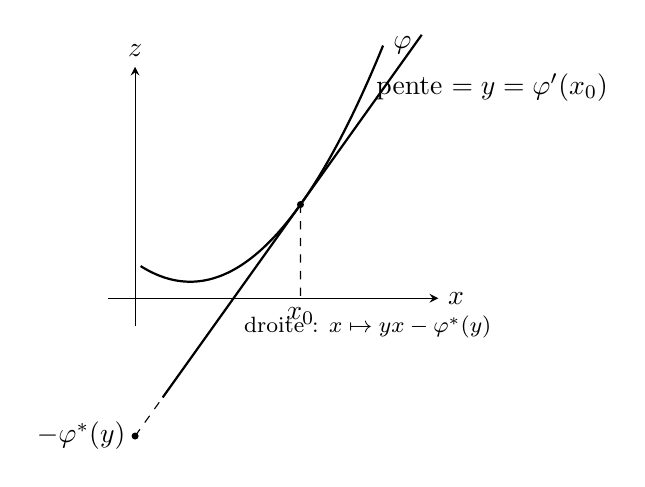
\begin{tikzpicture}[scale=0.7, >=stealth]

  % === Axes ===
  \draw[->] (-0.5, 0) -- (5.5, 0) node[right] {$x$};
  \draw[->] (0, -0.5) -- (0, 4.2) node[above] {$z$};

  % === Convex curve phi(x) = (x-1)^2 + 0.3 ===
  \draw[thick, domain=0.1:4.5, smooth, samples=100]
    plot (\x, {0.35*(\x-1)^2 + 0.3})
    node[right] {$\varphi$};

  % === Tangency point x_0 = 3 ===
  % phi(3)  = 0.35*(3-1)^2 + 0.3 = 0.35*4 + 0.3 = 1.7
  % phi'(3) = 0.7*(3-1) = 1.4  --> slope y = 1.4
  \coordinate (P) at (3, 1.7);

  % === Tangent line at x_0=3: z = y*(x - x_0) + phi(x_0) = 1.4*(x-3) + 1.7 ===
  % z = 1.4*x - 4.2 + 1.7 = 1.4*x - 2.5
  % At x=0: z = -2.5  -->  y-intercept = -phi*(y) = -2.5, so phi*(y)=2.5
  \draw[thick, domain=0.5:5.2, smooth]
    plot (\x, {1.4*\x - 2.5});

  % === Mark tangency point ===
  \filldraw (P) circle (1.5pt);

  % === Dashed lines from tangency point to axes ===
  \draw[dashed, thin] (P) -- (3, 0) node[below] {$x_0$};

  % === Label: slope annotation ===
  \node[above right] at (4.2, 3.4) {pente $= y = \varphi'(x_0)$};

  % === Label on y-axis: -phi*(y) ===
  % The tangent line at x=0 gives z = -2.5
  \draw[dashed, thin] (0, -2.5) -- (1.8, -2.5+1.4*1.8);
  \filldraw (0, -2.5) circle (1.5pt);
  \node[left] at (0, -2.5) {$-\varphi^*(y)$};

  % === Annotation: equation of the tangent line ===
  \node[below right] at (1.8, -0.15) {%
    \footnotesize droite : $x \mapsto yx - \varphi^*(y)$%
  };

\end{tikzpicture}\end{center}
    \end{df}

    \begin{prop}{}{}
        \begin{enumerate}
            \item $\varphi^*$ est toujours une fonction convexe
            \item Si $\varphi$ est $\Cr^2$ sur son domaine de définition et $\varphi\to +\infty$ aux bords du domaine, alors $\varphi=(\varphi^*)^*$
        \end{enumerate}
    \end{prop}

    \begin{proof}
        \begin{enumerate}
            \item Soit $p\in [0,1],y_1,y_2$
            \begin{align*}
                p\varphi^*(y_1)+(1-p)\varphi^*(y_2)&=p\sup_{x_1}(x_1 y_1-\varphi(x_1))+(1-p)\sup_{x_2}(x_2y_2-\varphi(x_2))\\
                &\ge \sup_x\left(x(py_1+(1-p)y_2)-\varphi(x)\right)=\varphi^*(py_1+(1-p)y_2)
            \end{align*}
            \item On remarque que sous ces hypothèses, $\varphi'$ est une bijection du domaine de définition de $\varphi$ dans $\R$.\\
            Pour $y$ donné, on suppose que le sup est atteint en un point $x$, $\varphi^*(y)=xy-\varphi(x)$. On dérive en x: $\varphi'(x)=y$ donc $x=(\varphi')^{-1}(y)$ et $\varphi^*(y)=y\left(\varphi'\right)^{-1}(x)-\varphi\left((\varphi')^{-1} (y)\right)$. On dérive,
            \[\left(\varphi^*\right)'(y)=\left(\varphi'\right)^{-1}(y)+y\frac{1}{\varphi''\left((\varphi'^{-1})(y)\right)}-\varphi'\left((\varphi')^{-1}\right)(y)\frac{1}{\varphi''\left((\varphi'^{-1})(y)\right)}\]
            D'où $(\varphi^*)'(y)=\left(\varphi'\right)^{-1}(y)$. En réappliquant à $\varphi^*$, on a
            \begin{align*}
                \left(\varphi^{**}\right)'(x)&=\left(\left(\varphi^*\right)^{-1}\right)(x)\\
                &=\varphi'(x)
            \end{align*}
            On doit vérifier:
            \begin{itemize}
                \item Le $\sup$ est atteint pour tout $y$
                \item $\varphi^*$ est $\Cr^2$
                \item $\displaystyle{\varphi^*(x) \underset{x\to \pm \infty}{\longrightarrow} +\infty}$
            \end{itemize}
            \vspace{0.5cm}
            \begin{itemize}
                \item Si le sup n'est pas atteint, on peut trouver $(x_n)_\nN$ tel que $x_n y-\varphi(x_n)\to \varphi*(y)=\sup_x xy-\varphi(y)$. Comme $\varphi$ est $C^\infty$ et $\to +\infty$ au bord de son domaine, $\varphi$ est minorée.\\
                Pour $y=0,\varphi*(0)=-\inf \varphi$ qui est atteint.\\
                Pour $y\neq 0$, tel que $\varphi*(y)<+\infty$, les $x_n$ doient rester dans un compact, on trouve $x$ tel que $\varphi*(y)=xy-\varphi(x)$ comme valeur d'adhérence des $x_n$.
                \item Si $\varphi''>0$ alors $\varphi'$ est strictement croissant et $(\varphi')^{-1}$ est aussi $C^1$.
                \item $\varphi*(y)\underset{y\to +\infty}{\longrightarrow}+\infty$ car $\varphi*(y)\ge y-\varphi(1)$\\
                $\varphi*(y)\underset{y\to -\infty}{\longrightarrow}+\infty$ car $\varphi*(y)\ge -y-\varphi(1)$
            \end{itemize}
        \end{enumerate}
    \end{proof}

    \begin{prop}{}{}
        Soit $(u_n)_n$ une suite sous-additive, c'est-à-dire telle que $\forall n,m, u_{n+m}\le u_n+u_m$. Alors $\frac{1}{n} u_n$ converge dans $\R\cup \{-\infty\}$
    \end{prop}

    \begin{proof}
        Montrons que $\limsup=\liminf$. Soit $(n_k)$ telle que $\dfrac{1}{n_k}u_{n_k}\to \liminf \dfrac{u_n}{n}$. Montrons que $\limsup \dfrac{u_n}{n}\le \dfrac{u_{n_k}}{n_k},\forall k$. On fixxe $k$, pour $N\gg n_k$, on écrit: $N=a n_k+b,k\le n_k$. $u_N\le a u_{n_k} +u_b$ par sous-additivité.
        \begin{align*}
            \dfrac{u_N}{N}&\le
        \end{align*}
    \end{proof}

    \begin{proof}
        Preuve du théorème de Cramer: On note $\displaystyle{s(r)=\sup_n \dfrac{1}{n}\log \Pa\left(\overline{X_m}\ge r\right)}$ avec $\displaystyle{\overline{X_m}=\dfrac{1}{m}\sum_{i=1}^{m}X_i}$.\\
        On va montrer que:
        \begin{enumerate}
            \item $s$ est concave
            \item $s=\lim \dfrac{1}{m}\ln \Pa\left(\overline{X_m}\ge r\right)$
            \item $-s=\varphi^*$
        \end{enumerate}
        \vspace{0.5cm}
        \begin{enumerate}
            \item Soit $p\in [0,1]\cap \Q,r_1,r_2$
            \begin{align*}
                ps(r_1)+(1-p) s(r_2)&=p\sup_{m_1}\dfrac{1}{m_1} \ln \Pa\left( \overline{X_{m_1}}\ge r_1\right)+(1-p)\sup_{m_2}\dfrac{1}{m_2}\ln \Pa\left(\overline{X_{m_2}}\ge r_2\right)\\
                \Pa\left(\overline{X_N}\ge pr_1 +(1-p)r_2\right)&\ge \Pa\left(\overline{X_{pN}}\ge r_1\text{ et }\dfrac{1}{(1-p)N} \sum_{pN+2}^{N^2} X_i \ge r_2\right)\\
                &\ge \Pa \left( \overline{X_{pN}}\ge r_1\right)\Pa\left(\overline{X_{pN+2}}\ge r_2\right)
            \end{align*}
            On repasse à $\dfrac{1}{N}\ln$. On étend la convexité à $p$ irrationnel car $\Pa \left(\overline{X_n}\ge r\right)$ est monotone en $r$.
            \item On vérifie que $u_n=\dfrac{1}{n}\ln \Pa\left(\overline{X_n}\ge r\right)$ est sous-additif. Même argument que pour la convexité.
            \[\Pa\left(\overline{X_{n+m}}\ge r\right)\ge \Pa\left(\overline{X_n}\ge r\right)\Pa\left(\overline{X_m}\ge r\right)\]
        \end{enumerate}
    \end{proof}

    \section{Théorème de Cramér dans $\R^d$}

    On cherche à comprendre les grandes déviations pour $\sum X_i$ avec $X_i$ i.i.d. à valeur dans $\R^d$.

    \begin{df}{}{}
        On dit qu'une suite de variables $S_n$ satisfait un principe de grande déviation si il existe une suite $v_n$ et une fonction $\funto{I}{\R^d}{[0,+\infty]}$ dont les ensembles de niveaux sont compacts $(\forall y<+\infty,\{x, I(x)\le y\}\text{ est compact})$
        \begin{itemize}
            \item $\forall O$ ouvert,
            \[\liminf \frac{1}{v_n} \log \left( \Pa\left(\frac{S_n}{n}\in O\right)\right)\ge -\inf_{s\in O} I(s)\]
            \item $\forall F$ fermé,
            \[\limsup \frac{1}{v_n} \log \left( \Pa\left(\frac{S_n}{n}\in F\right)\right)\le -\inf_{s\in F} I(s)\]
        \end{itemize}
    \end{df}

    \begin{tm}{Théorème de Cramer dans $\R^d$}{}
        Soit $X_i$ i.i.d. tel que $\varphi(\lambda):= \log \left(\Ea\left(e^{\lambda\cdot X}\right)\right)$ soit fini au voisinage de $O$.\\
        $S_n=\sum X_i$ satisfait un principe de grandes déviations de vitesse $v$ et de fonction de taux
        \[I(x)=\varphi^*(x):=\sup_\lambda \lambda\cdot x-\varphi(\lambda)\]
    \end{tm}

    \section{Théorème de Sanov}

    On considère une suite $X_n$ i.i.d. . On pose $\displaystyle{ \mu_n=\frac{1}{n} \sum_{i=1}^{n}\delta_{X_i}}$ la mesure empirique (variable aléatoire à valeurs dans l'espace des mesures).
    \[\mu_n(E)=\frac{1}{n} \left|\{i,X_i\in E\}\right|\]

    \begin{df}{}{}
        L'entropie relative à une mesure $\mu$ est la fonction:
        \[\fundf{\Mr(\Omega)}{\R}{\nu}{\cho{+\infty\text{ si $\nu$ n'est pas absoluement continue par rapport à $\mu$}\\ \int \rho(x)\log(\rho(x))\, d\mu(x)\text{ si $\dfrac{d\nu}{d\mu}=\rho$}}}\]
    \end{df}

    \begin{tm}{Théorème de Sanov}{}
        $\mu_n$ satisfait un principe de grande déviation de vitesse $n$ de fonction de taux
        \[I=\text{Ent}_{\text{loi de $X_1$}}\]
    \end{tm}

    \begin{proof}
        Idée de preuve: Cas où l'espace $\Omega=\{1,\ldots,k\}$ est fini, c'est à dire les variables $X_i$ sont à valeurs dans un ensemble fini.
        \[\mu_n=\sum_{l=1}^{k}\delta_l\dfrac{\left|\{i,X_i=l\}\right|}{n}\]
        On observe que $(\Nr_1,\ldots,\Nr_k)$ suit une loi multinomiale de paramètre $\Pa(X=1),\ldots,\Pa(X=k),n$.\\
        On note $p_1=\Pa(X=1),\ldots,p_k=\Pa(X=k)$
        \[\Pa\left(N_1=\alpha_1 n,\ldots,N_k=\alpha_k n\right)=\dfrac{n!}{\prod (\alpha_l n)!} \prod p_l^{\alpha_l n}\]
        Or, $\displaystyle{(\alpha n)! \underset{\text{Stirling}}{\sim}\left(\dfrac{\alpha n}{e}\right)^{\alpha n}= e^{\alpha n \ln (\alpha n) -\alpha n \ln l+ p(n)}}$. D'où
        \begin{align*}
            \Pa(N_1=\alpha_1 n,\ldots, N_k=\alpha_k n)&\sim e^{n\log n -n\log l-\sum_l n\alpha_l \ln (\alpha_l n)+\sum \alpha_l n \log p_l +\alpha_l n\log l}\\
            &\sim e^{-n \sum_l \alpha_l \ln \left(\dfrac{\alpha_l}{p_l}\right)}
        \end{align*}
        Cela conclut la preuve dans le cas d'un espace $\Omega$ fini.
    \end{proof}

    \subsubsection*{Réinterprétation du théorème de Cramer en dimension 1}

    Question: On se donne une loi $p$ centrée. Comment / Peut-on trouver $\cho{\text{ la}\\ \text{ une}}$ loi $q$ d'espérance $c$ qui minimise $\displaystyle{\text{Ent}_p(q)}$ ? On cherche $q$ sous la forme $\rho p$.\\
    Optimisation sous contrainte linéaire $\displaystyle{ \cho{\int x\rho( x)\, dp=c \\ \int \rho(x)\, dp=1}}$.
    \[\text{Ent}_p (\rho+\epsilon)-\text{Ent}_p (\rho)=\int (\rho+\epsilon)\log (\rho+\epsilon)\, dp -\int \rho \, dp=\int \epsilon \ln \rho +\rho \cdot \dfrac{\epsilon}{\rho} \, dp\]
    Si on choisit $\epsilon$ de sorte à ce que $(\rho+\epsilon)_p$ soit une proba. On a:
    \[\int \epsilon \, dp=0 \text{ (ce qu'on voulait)}\]
    \[\text{Ent}_p (\rho+\epsilon)-\text{Ent} (\rho)\sim \int \epsilon \ln \rho\]
    Pour le $\rho$ optimal, le gradient doit être orthogonal à l'espace où on optimise.\\
    On veut ici $\displaystyle{\int \epsilon \ln \rho \, dp=\text{cste }\int \epsilon \cdot x\, dp\implies \log \rho=\text{cste }x\iff \rho=e^{\lambda x}}$.\\
    \[\nabla \text{Ent} (\rho)\text{ est orthogonal à }A\iff \nabla \text{Ent$=$ cste}\vect{ n_A}\iff \vect{a}x=c\qquad A=\{x,b(x)=c\}\]
    \begin{align*}
        \partial_v \text{Ent} (\rho)&= v\cdot \nabla \text{Ent}\\
        &= v\cdot \vect{n_A}\cdot \text{cste}
    \end{align*}
\end{document}